%\setbeamertemplate{navigation symbols}{}
%\beamertemplatenavigationsymbolsempty

\setcounter{part}{4}

%%% \showfromto{5}{5}

\begin{document}

  % ------------------------------------------------------------------------------------------
  \begin{frame}
    \titlepage
    \note{
      \uzz{8:30}{11.1.\ $\to$ Folie 23}
      
      \parII
      \textbf{TODO:}~ siehe Verbesserungsvorschläge in TODO.txt
      
      \par
    }
  \end{frame}

  % ------------------------------------------------------------------------------------------
  \begin{frame}
    \frametitle{Überblick}

    \Bmph{Computation Tree Logic (CTL)}
    \begin{Itemize}
      \item
        Grenzen von LTL:~
        kann nicht über Pfade quantifizieren
        \par\smallskip
      \item
        Berechnungsbäume und CTL
        \par\smallskip
      \item
        Ausdrucksvermögen von LTL und CTL im Vergleich
        \par\smallskip
      \item
        Model-Checking mit CTL
    \end{Itemize}

    \par\bigskip
    \Bmph{Büchi-Automaten auf unendlichen Bäumen}
    \begin{Itemize}
      \item
        Definitionen und Beispiele
        \par\smallskip
      \item
        äquivalente Automatenmodelle:~ Muller-, Paritätsautomaten
        \par\smallskip
      \item
        Abschlusseigenschaften;\\
        Komplementierung von Muller-Automaten~~\Danger
    \end{Itemize}

    \note{
      \textbf{8:30}
      
      \par
    }
  \end{frame}

  % ------------------------------------------------------------------------------------------
  \begin{frame}
  \frametitle{Überblick}
    \tableofcontents
    \note{
      \textbf{8:32}
      
      \par
    }
  \end{frame}
  
  % ==============================================================================================
  % ==============================================================================================
  \section[\protect\emph{Model-Checking CTL}]{\protect\emph{Model-Checking mit CTL}}
  % ------------------------------------------------------------------------------------------
\begin{frame}
  \frametitle{Erinnerung an LTL\hfill {\normalsize\emph{(Linear Temporal Logic)}}}

  \begin{Itemize}
    \item%<+->
      System gegeben als Kripke-Struktur $\calS = (S,S_0,R,\ell)$
      \par\smallskip
    \item%<+->
      LTL-Formel $\varphi_E$ beschreibt Pfade,
      die Eigenschaft $E$ erfüllen
      \par\smallskip
%         \item<+->
%           benutzt dafür Operatoren $F,G,X,U$ \hfill{\footnotesize (auch üblich: $\Diamond,\Box,\bigcirc,U$)}
%           \par\smallskip
    \item%<+->
      Beispiel:\\
      "`Wenn Fehler auftritt, ist er nach endlicher Zeit behoben."'
      \par\smallskip
      $G(e \to F \neg e)$ \hfill {\footnotesize ($e \in \PROP$ steht für "`Error"')}
      \par\smallskip
    \item%<+->
      Umwandlung $\varphi_E$ in GNBA $\Aut{A}_E$,
      der zulässige Pfade beschreibt
      \par\smallskip
    \item%<+->
      lösen damit Model-Checking-Problem:
      \begin{Itemize}
        \item
          Gilt $E$ für \emph{alle} Pfade ab $S_0$ in \calS\,?\\
          \Bmph{(universelle Variante)}
        \item
          Gilt $E$ für \emph{mindestens einen} Pfad ab $S_0$ in \calS\,?\\
          \Bmph{(existenzielle Variante)}
      \end{Itemize}
  \end{Itemize}

  \par\bigskip
%       \uncover<+->{%
    \begin{footnotesize}
      LTL 1977 eingeführt durch Amir Pnueli, 1941-2009, \\
      israelischer Informatiker (Haifa, Weizmann-Inst., Stanford, Tel Aviv, New York)
      \par
    \end{footnotesize}

%       }
  \note{
    \textbf{8:33}
    
    \par
  }
\end{frame}

% ------------------------------------------------------------------------------------------
\begin{frame}
  \frametitle{Grenzen von LTL}

  "`LTL-Formel $\varphi_E$ beschreibt Pfade, die Eigenschaft $E$ erfüllen"'

  \par\bigskip
  \Bmph{Nicht ausdrückbar:}~ zu jedem Zeitpunkt ist es immer \emph{möglich},\\
  die Berechnung auf eine gewisse Weise fortzusetzen

  \par\bigskip
%       \uncover<2->{%
    \Bmph{Beispiel:}~~
    "`Wenn ein Fehler auftritt,\\
    ist es \emph{möglich}, ihn nach endlicher Zeit zu beheben."'
    \par\smallskip
    $G(e \to F \neg e)$ ~oder~ $GF\neg e$ ~sind
    \begin{Itemize}
      \item
        zu stark in Verbindung mit universellem Model-Checking \Tafel
      \item
        zu schwach in Verbindung mit existenziellem MC \TafelForts
    \end{Itemize}
%       }

  \note{
    \textbf{8:34 bis 8:46}
    
    \par
  }
\end{frame}

% ------------------------------------------------------------------------------------------
\begin{frame}
  \frametitle{Ein Fall für CTL\hfill {\normalsize\emph{(Computation Tree Logic)}}}

  \Bmph{Abhilfe:}~ Betrachten Berechnungsbäume statt Pfaden

  \par\bigskip
  Sei also $\calS = (S,S_0,R,\ell)$ eine Kripke-Struktur

  \par\bigskip
  \Bmph{Berechnungsbaum} für $s_0 \in S_0$
  \begin{Itemize}
    \item
      entsteht durch "`Auf{}falten"' von \calS in $s_0$
    \item
      enthält \emph{alle unendlichen} Pfade, die in $s_0$ starten
      \begin{Itemize}
        \item[] d.\,h.:
          jeder Zustand $s \in S$ hat als Kinder\\
          alle seine Nachfolgerzustände aus \calS
      \end{Itemize}
  \end{Itemize}

  \par\bigskip
  $\calS$ ist eine endliche Repräsentation aller $\infty$ Berechnungsbäume

%  \par\bigskip
%  \Gmph{Beispiel:} siehe nächste Folie \& Tafel \Tafel
%
  \note{
    \textbf{8:46}
    
    \par
  }
\end{frame}

% ------------------------------------------------------------------------------------------
\begin{frame}
  \label{fra:bsp_mikrowelle}
  \frametitle{Beispielstruktur Mikrowelle}

  \begin{center}
    \begin{minipage}[b]{.7\textwidth}
      \includegraphics[angle=270,width=\linewidth]{img/mc_microwave.jpg}\\
      {\footnotesize aus: E.\,M.\ Clarke et al., Model Checking, MIT Press 1999}
    \end{minipage}
  
    \par\vspace*{-\baselineskip}
    \Tafel
  \end{center}

  \note{
    \textbf{8:47 bis 8:54}
    
    \par
  }
\end{frame}

% ------------------------------------------------------------------------------------------
\begin{frame}
  \frametitle{CTL intuitiv}

  CTL enthält \Bmph{Pfadquantoren $A$, $E$:}
  \par\smallskip
  Operatoren, die über \Bmph{alle} oder \Bmph{einige} Berechnungen sprechen, \\
  die in einem bestimmten Zustand beginnen

  \par\bigskip
  \uncover<2->{%
    \Bmph{Beispiel:}~ $AGEF\neg e$
    \par\smallskip
    \qquad Für alle Berechnungen, die hier starten ($A$), \\
    \qquad gibt es zu jedem Zeitpunkt in der Zukunft ($G$) \\
    \qquad eine Möglichkeit, die Berechnung fortzusetzen ($E$), \\
    \qquad so dass irgendwann in der Zukunft ($F$) \\
    \qquad kein Fehler auftritt ($\neg e$)
  }

  \par\bigskip
  \uncover<3->{%
    \begin{footnotesize}
      CTL 1981 eingeführt durch\\
      \quad Edmund M.\ Clarke, ${}^*$1945, Informatiker, Carnegie Mellon Univ. (Pittsburgh)\\
      \quad E.\ Allen Emerson, ${}^*$1954, Informatiker, Univ.\ of Texas, Austin, USA\\
      (beide Turing-Award-Träger 2007)
      \par
    \end{footnotesize}
  }

  \note{
    \textbf{8:54}
    
    \par
  }
\end{frame}

% ------------------------------------------------------------------------------------------
\begin{frame}
  \frametitle{CTL exakt}

  Trennung von Zustands- und Pfadformeln:

  \par\bigskip
  \Bmph{Zustandsformeln} drücken Eigenschaften eines Zustandes aus
  \[
    \zeta ::= p \mid \zeta_1 \land \zeta_2 \mid \zeta_1 \lor \zeta_2 \mid \neg \zeta \mid E\psi \mid A\psi
  \]
  \begin{small}
    \qquad
    ($p$: Aussagenvariable;\hfill
    $\zeta,\zeta_1,\zeta_2$: Zustandsformeln;\hfill
    $\psi$: Pfadformel)
    \par
  \end{small}

  \par\bigskip
  \uncover<2->{%
    \Bmph{Pfadformeln} drücken Eigenschaften eines Pfades aus
    \[
      \psi ::= F\zeta \mid G\zeta \mid X\zeta \mid \zeta_1 \mathbin{U} \zeta_2
    \]
    \begin{small}
      \qquad
      \hfill
      ($\zeta,\zeta_1,\zeta_2$: Zustandsformeln)
      \par
    \end{small}
  }

  \par\bigskip
  \uncover<3->{%
    $\leadsto$ in \Bmph{zulässigen} CTL-Formeln muss
    \begin{Itemize}
      \item
        \mbox{\scalebox{.96}[1]{jeder Pfadquantor von einem temporalen Operator gefolgt werden}\hspace*{-10mm}}
      \item
        jeder temporale Operator direkt einem Pfadquantor folgen
    \end{Itemize}

  }

  \note{
    \textbf{8:56}
    
    \par
  }
\end{frame}

% ------------------------------------------------------------------------------------------
\begin{frame}
  \frametitle{Quiz: zulässige Formeln}

  Zur Erinnerung:
  \begin{align*}
    (ZF)\quad \zeta & ::= p \mid \zeta_1 \land \zeta_2 \mid \zeta_1 \lor \zeta_2 \mid \neg \zeta \mid E\psi \mid A\psi \\
    (PF)\quad \psi  & ::= F\zeta \mid G\zeta \mid X\zeta \mid \zeta_1 \mathbin{U} \zeta_2
  \end{align*}

  \par\bigskip
  \Emph{Quizfrage:} Welche der folgenden Formeln sind zulässig?
%       \begin{Itemize}
%         \item<+->
%           $p \land q$
% %           \uncover<+->{\YES}
% %         \item<+->
%           \quad
%           $EFp$
% %           \uncover<+->{\YES}
% %         \item<+->
%           \quad
%           $AXp$
%           \quad
%           \uncover<+->{\YES}
%         \item<+->
%           $E(p \mathbin{U} q)$
%           \quad
%           \uncover<+->{\YES}
%         \item<+->
%           $A((p \lor \neg p) \mathbin{U} q)$
%           \quad
% %           \uncover<+->{\YES}
% %           \quad
% %           \uncover<+->{(äquivalent zu $AFq$)}
%           \uncover<+->{%
%             \YES
%             \quad
%             (äquivalent zu $AFq$)
%           }
%         \item<+->
%           $E(p \lor AXq)$
%           \quad
%           \uncover<+->{\NO}
%         \item<+->
%           $EX(p \lor AXq)$
%           \quad
%           \uncover<+->{\YES}
%         \item<+->
%           $EF(p \mathbin{U} q)$
%           \quad
%           \uncover<+->{\NO}
%         \item<+->
%           $EFA(p \mathbin{U} q)$
%           \quad
%           \uncover<+->{\YES}
%       \end{Itemize}
  \begin{center}
    \begin{tabular}{@{}lll@{}}
      \uncover<+->{$p \land q$ \quad $EFp$ \quad $AXp$} & \uncover<+->{\YES} &                                    \\[2pt]
      \uncover<1->{$E(p \mathbin{U} q)$}                & \uncover<+->{\YES} &                                    \\[2pt]
      \uncover<1->{$A((p \lor \neg p) \mathbin{U} q)$}  & \uncover<+->{\YES  & (äquivalent zu $AFq$)}             \\[2pt]
      \uncover<1->{$E(p \lor AXq)$}                     & \uncover<+->{\NO   & ($E$ nicht gefolgt von $F,G,X,U$)} \\[2pt]
      \uncover<1->{$EX(p \lor AXq)$}                    & \uncover<+->{\YES} &                                    \\[2pt]
      \uncover<1->{$EF(p \mathbin{U} q)$}               & \uncover<+->{\NO   & ($U$ folgt nicht $E$ oder $A$)}    \\[2pt]
      \uncover<1->{$EFA(p \mathbin{U} q)$}              & \uncover<+->{\YES} &
    \end{tabular}
  \end{center}

  \note{
    \textbf{9:00}
    
    \textbf{Als Aufgabe, 2\,min Nachdenken, 2\,min Auf"|lösung $\leadsto$ bis 9:04}
    
    \par
  }
\end{frame}

\newlength{\leftbox}
\settowidth{\leftbox}{$\Paths(s):$}
% ------------------------------------------------------------------------------------------
\begin{frame}
  \frametitle{CTL-Semantik}

  CTL-Formeln werden über \Emph{Zuständen und Pfaden} von Kripke-Strukturen
  $\calS = (S,S_0,R,\ell)$ interpretiert

  \par\bigskip
  \Bmph{Schreibweisen}
  \begin{Itemize}
    \item
      $s \models \zeta$\quad für Zustände $s \in S$ und Zustandsformeln $\zeta$
    \item
      $\pi \models \psi$\quad für Pfade $\pi$ und Pfadformeln $\psi$
  \end{Itemize}

  \par\bigskip
  \Bmph{Hilfsbegriffe}
  \begin{Itemize}
    \item
      \parbox{\leftbox}{$\Paths(s)$:}\quad Menge aller Pfade, die in Zustand $s$ beginnen
    \item
      \parbox{\leftbox}{$\pi[i]$:}\quad $i$-ter Zustand auf dem Pfad $\pi$\\
      \parbox{\leftbox}{~}\quad         d.\,h.\ wenn $\pi=s_0s_1s_2\dots$, dann $\pi[i] = s_i$
  \end{Itemize}

  \note{
    \textbf{9:04}

    \par
  }
\end{frame}

% ------------------------------------------------------------------------------------------
\begin{frame}
  \frametitle{CTL-Semantik}

  Sei $\calS = (S,S_0,R,\ell)$ eine Kripke-Struktur.

  \begin{Definition}
    \Bmph{Erfülltheit von Zustandsformeln} in Zuständen $s \in S$
    \par\medskip
    \begin{tabular}{@{\quad}lll@{}}
        $s \models p$                     & falls & $p \in \ell(s)$, für alle $p \in \PROP$             \\[2pt]
        $s \models \lnot\zeta$            & falls & $s \not\models \zeta$                               \\[2pt]
        $s \models \zeta_1 \land \zeta_2$ & falls & $s \models \zeta_1$ und $s \models \zeta_2$
                                                    \quad~\, {\small (analog für $\zeta_1 \lor \zeta_2$)} \\[2pt]
        $s \models E\psi$                 & falls & $\pi \models \psi$ für ein $\pi \in \Paths(s)$      \\[2pt]
        $s \models A\psi$                 & falls & $\pi \models \psi$ für alle $\pi \in \Paths(s)$
    \end{tabular}

    \par\medskip
    \uncover<2->{%
      \Bmph{Erfülltheit von Pfadformeln} in Pfaden $\pi$ in $\calS$
      \par\medskip
      \begin{tabular}{@{\quad}lll@{}}
          $\pi \models X\zeta$              & falls & $\pi[1] \models \zeta$
                                                    \qquad\qquad\, {\small (analog für $F\zeta$ und $G\zeta$)}                  \\[2pt]
          $\pi \models \zeta_1\,U\,\zeta_2$ & falls & $\pi[\;\!j] \models \zeta_2$ für ein $j \geqslant 0$                  \\
                                            &       & und $\pi[k] \models \zeta_1$ für alle $k$ mit $0 \leqslant k < j$
      \end{tabular}
    }
  \end{Definition}

  \par\smallskip
  \uncover<3->{%
%         (Die Fälle $\zeta_1\lor\zeta_2$, $F\zeta$, $G\zeta$ sind analog.)
    Schreiben\quad $\calS \models \zeta$\quad falls\quad $s_0 \models \zeta$ für alle $s_0 \in S_0$
  }

  \note{
    \textbf{9:06}
    
    \par
  }
\end{frame}

% ------------------------------------------------------------------------------------------
\begin{frame}
  \frametitle{Zurück zu unseren Beispielen: Spezifikationen in CTL}

  \Bmph{Beispiel Nebenläufigkeit}
  \begin{Itemize}
    \item
%           Es kommt nie vor,\\
      Beide Teilprogramme sind nie zugleich im kritischen Bereich.
      \par\smallskip
      $AG\neg (p_{12} \land p_{22})$ \hfill {\footnotesize ($p_i \in \PROP$: "`Programmzähler in Zeile $i$"')}
      \par\smallskip
    \item<2->
      Jedes Teilprog.\ kommt beliebig oft in seinen krit.\ Bereich.
      \par\smallskip
      $AGAF p_{12} \land AGAF p_{22}$
      \par\smallskip
    \item<3->
      Jedes Teilprog.\ \emph{kann} beliebig oft in seinen kB kommen.
      \par\smallskip
      $AGEF p_{12} \land AGEF p_{22}$
  \end{Itemize}

  \par\bigskip
  \uncover<4->{%
    \Bmph{Liveness properties:}
    \par\smallskip
    $AG\zeta$ besagt: "`$\zeta$ ist in allen Berechnungen immer wahr"'
    \par\smallskip
    $AGAF\zeta$ besagt: "`$\zeta$ ist in allen Berechnungen $\infty$ oft wahr"'
    \par\smallskip
    $AGEF\zeta$ besagt: "`jede begonnene Berechnung kann so fortge-\\
    \hspace*{28mm}setzt werden, dass $\zeta$ irgendwann wahr wird."'
  }

  \note{
    \textbf{9:10}
    
    \par
  }
\end{frame}

% ------------------------------------------------------------------------------------------
\begin{frame}
  \frametitle{Zurück zu unseren Beispielen: Spezifikationen in CTL}

  \Bmph{Beispiel Mikrowelle}
  \begin{Itemize}
    \item
      "`Wenn Fehler auftritt, ist er nach endlicher Zeit behoben."'
      \par\smallskip
      $AG(e \to AF \neg e)$ \hfill {\footnotesize ($e \in \PROP$ steht für "`Error"')}
      \par\smallskip
    \item<2->
      "`Wenn Fehler auftritt, \emph{kann} er nach endl.\ Z.\ behoben werden"'
      \par\smallskip
      $AG(e \to EF \neg e)$
      \par\smallskip
    \item<3->
      "`Wenn die Mikrowelle gestartet wird, \\
      beginnt sie nach endlicher Zeit zu heizen."'
      \par\smallskip
      $AG(s \to AF h)$ \hfill {\footnotesize ($s,h \in \PROP$ stehen für "`Start"' bzw.\ "`Heat"')}
      \par\smallskip
    \item<4->
      "`Wenn die Mikrowelle gestartet wird, \\
      \emph{ist es möglich}, dass sie nach endlicher Zeit zu heizen beginnt."'
      \par\smallskip
      $AG(s \to EF h)$
      \par\bigskip
%         \emphitem<5->
%           $AG(\zeta_1 \to AF \zeta_2)$,~
%           $AG(\zeta_1 \to EF \zeta_2)$:~
%           \Bmph{progress properties}
  \end{Itemize}

  \par\medskip
  \uncover<5->{%
    \Bmph{Progress properties:}~
    $AG(\zeta_1 \to AF \zeta_2)$,~
    $AG(\zeta_1 \to EF \zeta_2)$~ bedeuten: \\
    \par\smallskip
    Wann immer $\zeta_1$ eintritt, ist nach endlicher Zeit $\zeta_2$ "`garantiert"'
  }

  \note{
    \textbf{9:12}
    
    \par
  }
\end{frame}

% ------------------------------------------------------------------------------------------
\begin{frame}
  \frametitle{Ausdrucksstärke von CTL versus LTL}
  
  \begin{definition}
    Seien $\zeta$ eine CTL-Zustandsformel und $\varphi$ eine LTL-Formel.
    
    \par\smallskip
    $\zeta$ und $\varphi$ sind \Bmph{äquivalent,} geschrieben \Bmph{$\zeta \equiv \varphi$,}
    wenn für alle Kripke-Strukturen $\Smc = (S,S_0,R,\ell)$ gilt:
    \begin{center}
      $\Smc \models \zeta$
      \quad gdw.\quad
      $\Smc \models \varphi$
    \end{center}
  \end{definition}

  \par\medskip
  \Bmph{Zur Erinnerung:}
  %
  \begin{Itemize}
    \item
      $\Smc \models \zeta$, wenn $s_0 \models \zeta$ für \Emph{alle} $s_0 \in S_0$
    \item
      $\Smc \models \varphi$, wenn $\pi,0 \models \varphi$ für \Emph{alle} $\pi \in \Paths(s_0)$ und \Emph{alle} $s_0 \in S_0$
  \end{Itemize}
  
  \note{
    \textbf{9:15: 5\,min Pause, dann 2\,min für Folie}
    
    \par
  }
\end{frame}

% ------------------------------------------------------------------------------------------
\begin{frame}
  \frametitle{Ausdrucksstärke von CTL versus LTL}

  \begin{lemma}
    $AFAGp \not\equiv FGp$
    \label{lem:AFAGp_not_equiv_FGp}
  \end{lemma}

  \uncover<2->{%
    \Bmph{Beweis.}~
    Betrachte Kripke-Struktur $\calS$:
%    \raisebox{-4pt}{\Fig0}%
    \begin{tikzpicture}[%
      node distance=12mm,>=Latex,baseline=-2pt,
      initial text="", initial where=below left,
      every state/.style={draw=black,thick,fill=none,inner sep=.8mm,minimum size=5mm},
      accepting/.style={double distance=1.5pt, double=white},
      every edge/.style={draw=black,thick}
    ]
      \node[state,initial] (s0)               {$s_0$};
      \node[state]         (s1) [right of=s0] {$s_1$};
      \node[state]         (s2) [right of=s1] {$s_2$};
      
      \path[->] (s0) edge              (s1)
                (s1) edge              (s2)
                (s0) edge [loop below] ()
                (s2) edge [loop below] ();
      
      \node () [above right=-1mm and -1mm of s0] {$p$};
      \node () [above right=-1mm and -1mm of s2] {$p$};
    \end{tikzpicture}
    
    \begin{Itemize}
      \item
        alle Pfade $\pi \in \Paths(s_0)$ erfüllen $FGp$
      \item<3->
        aber $\calS \not\models AFAGp$:
        \par\medskip
        \begin{tabular}{@{\quad}ll@{\qquad}l@{}}
          \uncover<4->{              & $s_0s_1s_2^\omega \not\models Gp$ & {\small wegen $p \notin \ell(s_1)$}              \\[1pt] }
          \uncover<5->{$\Rightarrow$ & $s_0 \not\models AGp$             & {\small weil $s_0s_1s_2^\omega \in \Paths(s_0)$} \\[1pt] }
          \uncover<6->{$\Rightarrow$ & $s_0^\omega \not\models FAGp$     & {\small weil $s_0^\omega$ nur aus $s_0$ besteht} \\[1pt] }
          \uncover<7->{$\Rightarrow$ & $s_0 \not\models AFAGp$           & {\small weil $s_0^\omega \in \Paths(s_0)$}               }
        \end{tabular}
    \end{Itemize}
    \uncover<8->{%
      \qed
    }
  }

  \note{
    \textbf{9:22}
    
    \par
  }
\end{frame}

% ------------------------------------------------------------------------------------------
\begin{frame}
  \frametitle{Ausdrucksstärke von CTL versus LTL}
  
  \begin{lemma}
    Sei $\zeta$ eine CTL-Zustandsformel und $\zeta'$ die LTL-Formel,
    die man durch Entfernen aller Pfadquantoren aus $\zeta$ erhält.
    Dann gilt:
    %
    \begin{center}
      $\zeta \equiv \zeta'$ oder es gibt keine zu $\zeta$ äquivalente LTL-Formel.
    \end{center}
    \par\vspace*{-.4\baselineskip}
    \label{lem:aequiv_LTL_Fmln}
  \end{lemma}

  \par
  \Bmph{Ohne Beweis.} (Clarke, Draghicescu 1988)
  
  \parII
  \uncover<2->{%
    \begin{lemma}
      \begin{Enumerate}
        \item[\Bmph{(1)}]
          Es gibt keine zu $AFAGp$ äquivalente LTL-Formel.
        \item[\Bmph{(2)}]
          Es gibt keine zu $FGp$ äquivalente CTL-Zustandsformel.
      \end{Enumerate}
    \end{lemma}
  }
  
  \parI
  \uncover<3->{%
    \Bmph{Beweis.}
    
    \parI
    \Bmph{(1)} folgt aus Lemmas~\ref{lem:AFAGp_not_equiv_FGp} und~\ref{lem:aequiv_LTL_Fmln}
  }

  \parI
  \uncover<4->{%
    \Bmph{(2)} siehe Tafel \Tafel~~~~~
    \par\vspace*{-\baselineskip}\qed
  }
  
  \note{
    \textbf{9:26 bis 9:38}
    
    \par
  }
\end{frame}

% ------------------------------------------------------------------------------------------
\begin{frame}
  \frametitle{Ausdrucksstärke von CTL versus LTL}
  
  Auch \Bmph{progress properties} sind \Emph{nicht} in LTL ausdrückbar:
  
  \begin{lemma}
    Sei $\zeta = AG(p \to EF p')$.
    Es gibt keine zu $\zeta$ äquivalente LTL-Formel.
  \end{lemma}

  \parI
  \uncover<2->{%
    \Bmph{Beweis.}
    Angenommen, es gebe LTL-Formel $\varphi \equiv \zeta$.
    
  }

  \parII    
  \uncover<3->{%
    Betrachte Kripke-Strukturen

    \par\vspace*{-.6\baselineskip}
    \begin{center}    
      $\Smc_1$
      \begin{tikzpicture}[%
        node distance=12mm,>=Latex,baseline=-2pt,
        initial text="", initial where=below left,
        every state/.style={draw=black,thick,fill=none,inner sep=.8mm,minimum size=5mm},
        accepting/.style={double distance=1.5pt, double=white},
        every edge/.style={draw=black,thick}
      ]
        \node[state,initial] (s0)               {$s_0$};
        \node[state]         (s1) [right of=s0] {$s_1$};
        
        \path[->] (s0) edge              (s1)
                  (s0) edge [loop below] ()
                  (s1) edge [loop below] ();
                  
        \node () [above right=-1mm and -1mm of s0] {$p$};
        \node () [above right=-1mm and -1mm of s1] {$p'$};
      \end{tikzpicture}
      \qquad
      $\Smc_2$
      \begin{tikzpicture}[%
        node distance=12mm,>=Latex,baseline=-2pt,
        initial text="", initial where=below left,
        every state/.style={draw=black,thick,fill=none,inner sep=.8mm,minimum size=5mm},
        accepting/.style={double distance=1.5pt, double=white},
        every edge/.style={draw=black,thick}
      ]
        \node[state,initial] (s2)               {$s_2$};
        
        \path[->] (s2) edge [loop below] ();
        
        \node () [above right=-1mm and -1mm of s2] {$p$};
      \end{tikzpicture}
    \end{center}
  }

  \par\vspace*{-.6\baselineskip}
  \uncover<4->{%
    Dann gilt $\Smc_1 \models \zeta$.
  }

  \parII
  \uncover<5->{%
    Also auch $\Smc_1 \models \varphi$.
  }
    
  \parII
  \uncover<6->{%
    Da $\Paths(s_2) \subseteq \Paths(s_0)$, gilt auch $\Smc_2 \models \varphi$.
  }

  \parII
  \uncover<7->{%
    Aber offensichtlich $\Smc_2 \not\models \zeta$.~ \lightning
    \qed
  }

  \note{
    \textbf{9:38}

    \par
  }
\end{frame}
  
% ------------------------------------------------------------------------------------------
\begin{frame}
  \frametitle{Ausdrucksstärke von CTL versus LTL}
  
  \par\bigskip
  \uncover<+->{%
    Erweiterung von LTL und CTL: \Bmph{CTL*}
    \par\vspace*{-2pt}
    {\footnotesize CTL*: 1986 von E.\ A.\ Emerson und J.\ Y.\ Halpern (${}^*$1953, Inform., Cornell)}
  }

  \note{
    \textbf{9:42}
    
    \par
  }
\end{frame}

% ------------------------------------------------------------------------------------------
\begin{frame}
  \frametitle{Model-Checking für CTL (Skizze)}

  \Bmph{Standard-Algorithmus} ("`bottom-up labelling"', ohne Automaten):

  \par\bigskip
  Eingabe: Kripke-Str.\ \calS, Zust.\ $s_0$, CTL-Zustandsformel $\zeta$
  \par
  Frage: $s_0 \models \zeta$\,?
  
  \par\bigskip
  Vorgehen:
  \begin{Itemize}
    \item<2->
      Stelle $\zeta$ als Baum dar\hspace*{\fill} (Bsp.\ siehe Tafel) \Tafel
    \item<3->
      Gehe Baum von unten nach oben durch\\
      und markiere Zustände $s$ in $\calS$ mit der jeweiligen Teilformel,\\
      wenn sie in $s$ erfüllt ist \TafelForts
    \item<4->
      Akzeptiere gdw.\ $s_0$ mit $\zeta$ markiert ist
  \end{Itemize}

  \par\bigskip
  \uncover<5->{%
    \Bmph{Komplexität:} \PT-vollständig \quad (LTL-MC: \PSPACE-vollständig)
    
    \parII
    \scalebox{.98}[1]{Dafür ist CTL-SAT \EXP-vollständig\quad (LTL-SAT: \PSPACE-vollst.).}
  }

  \note{
    \textbf{9:42 bis 9:53}
    
    \par
  }
\end{frame}

% ------------------------------------------------------------------------------------------
\begin{frame}
  \frametitle{Model-Checking für CTL mit Baumautomaten}

  \Bmph{Automatenbasierte Entscheidungsprozedur für CTL}
  \begin{Itemize}
    \item[\dots]
      basiert auf \Bmph{alternierenden Baumautomaten}\\[.4\baselineskip]
      \begin{small}
        (Erweiterung des Begriffs der nichtdeterminist.\ Baumautomaten; \\
        siehe Teil 5 der Vorlesung)
        \par
      \end{small}
%    \item
%      voraussichtlich in Teil 5 der Vorlesung anreißen %\\
%%           {\small (siehe V\,$+$\,Ü "`Verifikation unendlicher Systeme"', WS 13/14)}
  \end{Itemize}

  \par\bigskip
  \uncover<2->{%
    \Bmph{Verwandt:}
    \par\smallskip
    Automatenbasierte Entscheidungsprozedur für CTL*-\Emph{Erfüllbarkeit}
    \begin{Itemize}
      \item
        basiert auf nichtdeterministischen Rabin-Baumautomaten
      \item
        technisch aufwändige Konstruktion
      \item
        hier nicht behandelt %\\
    \end{Itemize}
  }

  \par\bigskip
  \uncover<3->{%
    \Bmph{Es folgt:}
    \begin{Itemize}
      \item[]
        Überblick "`klassische"' nichdeterministische Baumautomaten
    \end{Itemize}
  }

  \note{
    \textbf{9:53 bis 9:55, 5\,min Reserve.}
    
    \parIII
    CTL*-MC ist PSpace-vollst., CTL*-SAT 2ExpTime-vollst.\\
    Siehe Baier \& Katoen S.\ 430.
    
    \par
  }
\end{frame}



  % ==============================================================================================
  % ==============================================================================================
  \section[Baumautomaten]{Automaten auf unendlichen Bäumen}
  % ------------------------------------------------------------------------------------------
\begin{frame}
  \frametitle{Baumautomaten: Grundbegriffe}

  Betrachten \Bmph{unendlichen vollständigen Binärbaum}
  \begin{Itemize}
    \item
      Positionen: \emph{alle} Wörter aus $\{0,1\}^*$
    \item
      jeder Knoten $p$ hat linkes und rechtes Kind: $p0,p1$
    \item
      \Bmph{Tiefe} von Knoten $p$:\quad $|p|$
    \item
      \Bmph{Ebene} $k$: alle Knoten der Tiefe $k$
    \item
      $p_2$ ist \Bmph{Nachfolger} von $p_1$, geschrieben $p_1 \sqsubseteq p_2$,\\
      wenn $p_2=p_1p$ für ein $p \in \{0,1\}^*$
      \Tafel
  \end{Itemize}

  \par\medskip
  \uncover<2->{%
    \Bmph{Pfad}: Teilmenge $\pi \subseteq \{0,1\}^*$ mit $\varepsilon \in \pi$ und:
    \begin{Itemize}
%           \item
%             Wurzel $\varepsilon \in \pi$
      \item
        wenn $p \in \pi$, dann genau eins der Kinder $p0,p1$ in $\pi$
      \item
        $\forall k$: von allen Knoten der Ebene $k$ ist genau einer in $\pi$ \\
        \TafelForts
    \end{Itemize}
  }

  \par%\medskip
  \uncover<3->{%
    \Bmph{$\Sigma$-Baum $t$} (Alphabet $\Sigma$ ohne Stelligkeit): \\
    \begin{Itemize}
      \item[]
        Funktion $t : \{0,1\}^* \to \Sigma$
        \TafelForts
    \end{Itemize}
  }

  \note{%
    \textbf{16:00}
    
    \par
  }
\end{frame}

%% ------------------------------------------------------------------------------------------
%\begin{frame}
%  \frametitle{Skizzen zu den Grundbegriffen}
%
%  Positionen und Pfade im Binärbaum
%  \begin{center}
%    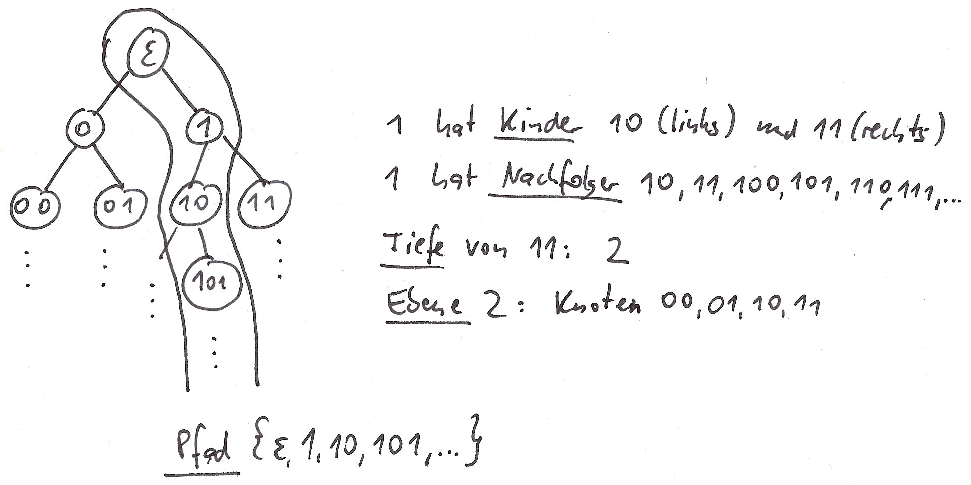
\includegraphics[scale=.5]{img/skizzen_baeume_1.pdf}
%  \end{center}
%
%  \par\bigskip
%%       Beispiel für einen $\Sigma$-Baum, $\Sigma=\{a,b\}$
%  Beispiel-$\Sigma$-Baum,\\
%  $\Sigma=\{a,b\}$
%  \par\vspace*{-2.1\baselineskip}
%  \hspace*{.3\textwidth}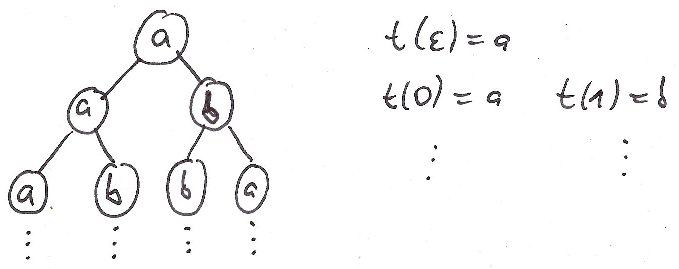
\includegraphics[scale=.5]{img/skizzen_baeume_2.pdf}
%
%  \note{~}
%\end{frame}

% ------------------------------------------------------------------------------------------
\begin{frame}
  \frametitle{Baumautomaten: etwas mehr Notation (1)}
  
  $\hat t = \Bmph{$t[p \to t_1]$}$:
  \par\smallskip
  der Baum, den man aus $t$ erhält, wenn man den Teilbaum,\\
  der in $p$ wurzelt, durch $t_1$ ersetzt

  \par\bigskip
  Skizze:
  \begin{center}
    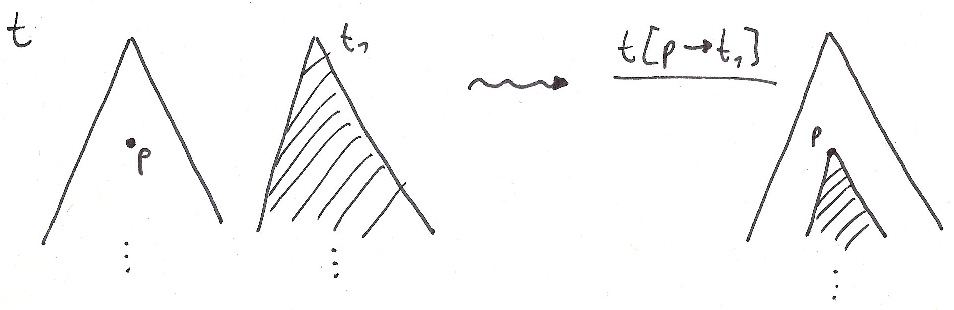
\includegraphics[scale=.5]{img/skizzen_baeume_3.pdf}
  \end{center}

  \par\bigskip
  exakte Beschreibung:
  \[
    \hat t(p') =
    \begin{cases}
      t_1(p'') & \text{wenn } p'=pp'' \\
      t(p')    & \text{wenn } p \not\sqsubseteq p'
    \end{cases}
  \]

  \note{%
    \textbf{16:08}
    
    \par
  }
\end{frame}

% ------------------------------------------------------------------------------------------
\begin{frame}
  \frametitle{Baumautomaten: etwas mehr Notation (2)}

  $\hat t = \Bmph{$a(t_0,t_1)$}$:
  \par\smallskip
  der Baum mit Wurzel $a$ und Teilbäumen $t_0,t_1$ in den Wurzelkindern $0,1$:

  \par\bigskip
  Skizze:
  \begin{center}
    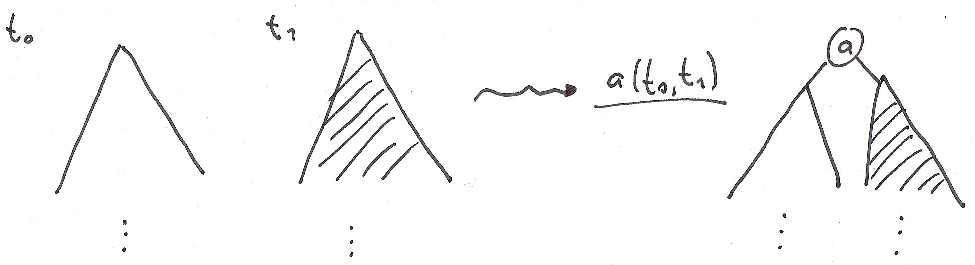
\includegraphics[scale=.5]{img/skizzen_baeume_4.pdf}
  \end{center}

  \par\bigskip
  exakte Beschreibung:
  \[
    \hat t(p) =
    \begin{cases}
      a        & \text{wenn } p=\varepsilon \\
      t_0(p')  & \text{wenn } p=0p'         \\
      t_1(p')  & \text{wenn } p=1p'
    \end{cases}
  \]

  \note{%
    \textbf{16:11}
    
    \par
  }
\end{frame}

% ------------------------------------------------------------------------------------------
\begin{frame}
  \frametitle{Baumautomaten: Definition}

  \begin{Definition}
    Ein \Bmph{nichtdeterministischer Büchi-Baumautomat (NBBA)} über $\Sigma$\\
    ist ein 5-$\!$Tupel
    $\Aut{A} = (Q, \Sigma, \Delta, I, F)$, wobei
    \begin{Itemize}
      \item
        $Q$ eine endliche nichtleere \Bmph{Zustandsmenge} ist,
      \item
        $\Sigma$ ein Alphabet ist
      \item
        $\Delta \subseteq Q \times \Sigma \times \uwave{Q \times Q}$ die \Bmph{Überführungsrelation} ist,
      \item
        $I \subseteq Q$ die Menge der \Bmph{Anfangszustände} ist,
      \item
        $F \subseteq Q$ die Menge der \Bmph{akzeptierenden Zustände} ist.
    \end{Itemize}
  \end{Definition}

  \par\bigskip
  \uncover<2->{%
    (entsprechen offenbar Top-down-Automaten)
  }

  \note{%
    \textbf{16:14}
    
    \par
  }
\end{frame}

% ------------------------------------------------------------------------------------------
\begin{frame}
  \frametitle{Muller- und Paritäts-Baumautomaten}

  \begin{Definition}
    Ein \Bmph{nichtdeterministischer Muller-Baumautomat (NMBA)} über $\Sigma$\\
    ist ein 5-$\!$Tupel
    $\Aut{A} = (Q, \Sigma, \Delta, I, \calF)$, wobei
    \begin{Itemize}
      \item
        $Q,\Sigma,\Delta,I$ wie für NBBAs sind
      \item
        $\calF \subseteq 2^Q$ die \Bmph{Akzeptanzkomponente} ist
    \end{Itemize}

    \par\bigskip
    \uncover<2->{%
      Ein \Bmph{nichtdeterministischer Paritäts-Baumautomat (NPBA)} über $\Sigma$\\
      ist ein 5-$\!$Tupel
      $\Aut{A} = (Q, \Sigma, \Delta, I, c)$, wobei
      \begin{Itemize}
        \item
          $Q,\Sigma,\Delta,I$ wie für NBBAs sind
        \item
          $c : Q \to \mathbb{N}$ die \Bmph{Akzeptanzkomponente} ist
      \end{Itemize}
    }
  \end{Definition}

  \par\bigskip
  \uncover<3->{%
    (Rabin- und Streett-Baumautomaten wie üblich definiert)
  }

  \note{%
    \textbf{16:15}
    
    \par
  }
\end{frame}

% ------------------------------------------------------------------------------------------
\begin{frame}
  \frametitle{Runs auf Baumautomaten}

  Run $=$ Markierung der Positionen in $\{0,1\}^*$ mit Zuständen,\\
  verträglich mit Anfangszuständen und Überführungsrelation

  \par\bigskip
  \uncover<2->{%
    \begin{Definition}
      Ein \Bmph{Run} eines NBBA (NMBA, NPBA) \Aut{A} auf einem $\Sigma$-Baum $t$\\
      ist eine Funktion $r : \{0,1\}^* \to Q$, so dass
      \begin{Itemize}
        \item
          $r(\varepsilon) \in I$;
        \item
          für alle $p \in \{0,1\}^*$ gilt: $\big(r(p), t(p), r(p0), r(p1)\big) \in \Delta$
      \end{Itemize}
    \end{Definition}
  }

  \par\bigskip
  \uncover<3->{%
    Erfolgreicher Run: verträglich mit Akzeptanzkomponente
  }

  \note{%
    \textbf{16:16}
    
    \par
  }
\end{frame}

%   \newlength{\leftbox}
%   \settowidth{\leftbox}{$x=\text{Parität}$;}
%   \newlength{\midbox}
%   \settowidth{\midbox}{$\textsl{Acc}=\calF$;}
%   % ------------------------------------------------------------------------------------------
%     \begin{frame}
%       \frametitle{Erfolgreiche Runs}
% 
%       Sei $r$ Run eines N$x$BAs \Aut{A} % auf einem $\Sigma$-Baum $t$
%       und $\pi$ ein Pfad
% 
%       \par\medskip
%       Betrachten wieder \Bmph{Unendlichkeitsmenge}
%       \[
%         \Inf(r,\pi) = \{q \in Q \mid r(p) = q \text{~für unendlich viele~} p \in \pi\}
%       \]
% 
%       \par%\bigskip
%       \begin{Definition}<2->      
%         Run $r$ des N$x$BA $\Aut{A}=(Q,\Sigma,\Delta,I,\textsl{Acc})$ ist \Bmph{erfolgreich}, falls
%         \begin{Itemize}
%           \item
%             \parbox{\leftbox}{$x=\text{Büchi}$;} \parbox{\midbox}{$\textsl{Acc}=F$;} für alle Pfade $\pi$:~
%             $
%               \Inf(r,\pi) \cap F \neq \emptyset
%             $
%           \item<3->
%             \parbox{\leftbox}{$x=\text{Muller}$;} \parbox{\midbox}{$\textsl{Acc}=\calF$;} für alle Pfade $\pi$:~
%             $
%               \Inf(r,\pi) \in \calF
%             $
%           \item<4->
%             \parbox{\leftbox}{$x=\text{Parität}$;} \parbox{\midbox}{$\textsl{Acc}=c$;} für alle Pfade $\pi$:
%             \[
%               \min\{c(q) \mid q \in \Inf(r,\pi)\} \text{~ist gerade}
%             \]%
%         \end{Itemize}
% 
%         \par\vspace*{-1.2\baselineskip}
%         \uncover<5->{%
%           $\Aut{A}$ \Bmph{akzeptiert} $t$, wenn es einen erfolgreichen Run von \Aut{A} auf $t$ gibt.
%         }
% 
%         \par\smallskip
%         \uncover<6->{%
%           \Bmph{$L_\omega(\Aut{A})$} $=$ $\{t \mid \Aut{A} \text{~akzeptiert~} t\}$
%         }
%       \end{Definition}
% 
%       \note{~}
%     \end{frame}

% ------------------------------------------------------------------------------------------
\begin{frame}
  \frametitle{Erfolgreiche Runs}

  Sei $r$ Run eines N$x$BAs \Aut{A} % auf einem $\Sigma$-Baum $t$
  und $\pi$ ein Pfad

  \par\smallskip
  Betrachten wieder \Bmph{Unendlichkeitsmenge}
  \[
    \Inf(r,\pi) = \{q \in Q \mid r(p) = q \text{~für unendlich viele~} p \in \pi\}
  \]

  \par
  \begin{Definition}<2->      
    \begin{Itemize}
      \item
        Run $r$ des NBBA $\Aut{A}=(Q,\Sigma,\Delta,I,F)$ ist \Bmph{erfolgreich}, falls
        \par\smallskip
        \Emph{für alle Pfade} $\pi$ gilt:~ $\Inf(r,\pi) \cap F \neq \emptyset$
        \par\smallskip
      \item<3->
        Run $r$ des NMBA $\Aut{A}=(Q,\Sigma,\Delta,I,\calF)$ ist \Bmph{erfolgreich}, falls
        \par\smallskip
        \Emph{für alle Pfade} $\pi$ gilt:~ $\Inf(r,\pi) \in \calF$
        \par\smallskip
      \item<4->
        Run $r$ des NPBA $\Aut{A}=(Q,\Sigma,\Delta,I,c)$ ist \Bmph{erfolgreich}, falls
        \par\smallskip
        \Emph{für alle Pfade} $\pi$ gilt:~ 
        $
          \min\{c(q) \mid q \in \Inf(r,\pi)\} \text{~ist gerade}
        $
    \end{Itemize}

%         \par\vspace*{-1.2\baselineskip}
  \end{Definition}

  \note{%
    \textbf{16:18}
    
    \parI
    Parity-Bedingung: in Aufgabe 4 auf Übungsblatt 4 war es max statt min \\
    -- macht aber keinen Unterschied; ggf.\ Nummerierung der Zustände "`umdrehen"'.
    
    \par
  }
\end{frame}

% ------------------------------------------------------------------------------------------
\begin{frame}
  \frametitle{Akzeptanz und erkannte Sprache}

  \dots\ sind wie üblich definiert:

  \par\bigskip
  \begin{Definition}
    Sei $\Aut{A}$ ein NBBA, NMBA oder NPBA,\\
    sei $t$ ein $\Sigma$-Baum und $L$ eine Menge von $\Sigma$-Bäumen.
    \begin{Itemize}
      \item
        $\Aut{A}$ \Bmph{akzeptiert} $t$,\\
        wenn es einen erfolgreichen Run von \Aut{A} auf $t$ gibt.
        \par\smallskip
      \item
        \Bmph{$L_\omega(\Aut{A})$} $=$ $\{t \mid \Aut{A} \text{~akzeptiert~} t\}$
        \par\bigskip
      \item
        $L$ heißt \Bmph{Büchi-erkennbar},\\
        wenn es einen NBBA $\Aut{A}$ gibt mit $L_\omega(\Aut{A})=L$.
        \par\smallskip
      \item
        Analog: \Bmph{Muller-erkennbar} und \Bmph{paritäts-erkennbar}
    \end{Itemize}
  \end{Definition}

  \note{%
    \textbf{16:20}
    
    \par
  }
\end{frame}

% ------------------------------------------------------------------------------------------
\begin{frame}
  \frametitle{Beispiele (Büchi)}

  \begin{Itemize}
    \item<+->
      NBBA $\Aut{A}=(\{A,B\},~\{a,b\},~\Delta,~\{A\},~\{A\})$ mit %\Tafel
      \[
        \Delta = \{~(A,a,A,A),~(B,a,A,A),~(A,b,B,B),~(B,b,B,B)~\}
      \]
      Skizze:
      \par\vspace*{-\baselineskip}
      \begin{center}
        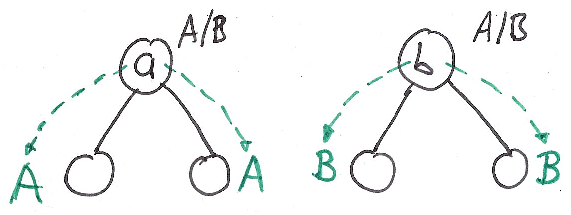
\includegraphics[scale=.5]{img/beispielautomaten_1.pdf}
      \end{center}

      \par\bigskip
      $L_\omega(\Aut{A})$ $=$
      \only<.|handout:0>{?}%
      \uncover<+->{$\{t \mid \text{jeder Pfad hat $\infty$ viele $a$'s}\}$}
      \par\bigskip
    \item<+->
      derselbe NBBA, aber mit $F=\{B\}$
      \par\smallskip
      $L_\omega(\Aut{A})$ $=$
      \only<.|handout:0>{?}%
      \uncover<+->{$\{t \mid \text{jeder Pfad hat $\infty$ viele $b$'s}\}$}
      \par\bigskip
    \item<+->
      derselbe NBBA, aber mit $F=\{A,B\}$
      \par\smallskip
      $L_\omega(\Aut{A})$ $=$
      \only<.|handout:0>{?}%
      \uncover<+->{$\{t \mid t \text{~ist ein $\Sigma$-Baum}\}$}
  \end{Itemize}

  \note{%
    \textbf{16:21}
    
    \par
  }
\end{frame}

% ------------------------------------------------------------------------------------------
\begin{frame}
  \frametitle{Beispiele (Büchi)}

  \begin{Itemize}
    \item<+->
      NBBA $\Aut{A}=(\{A,B,X\},~\{a,b\},~\Delta,~\{A\},~\{A,X\})$ mit $\Delta = $%\Tafel
%           \[
%             \begin{array}{rlll}
%               \text{mit~} \Delta = \{~ & (A,a,A,X),~ & (A,a,X,A), & \\
%                                        & (B,a,A,X),~ & (B,a,X,A), & \\[5pt]
%                                        & (A,b,B,X),~ & (A,b,X,B), & \\
%                                        & (B,b,B,X),~ & (B,b,X,B), & \\[5pt]
%                                        & (X,a,X,X),~ & (X,b,X,X)~ & \}
%             \end{array}
%           \]
      \par\medskip
      \begin{small}
        \mbox{$
          \begin{array}{@{}r@{~}l@{~~}l@{~~}l@{~~}l@{~~}l@{~}l@{}}
            \{ & (A,a,A,X),~ & (B,a,A,X),~ & (A,b,B,X),~ & (B,b,B,X),~ & (X,a,X,X), &    \\
               & (A,a,X,A),~ & (B,a,X,A),~ & (A,b,X,B),~ & (B,b,X,B),~ & (X,b,X,X)  & \}
          \end{array}
        $\hspace*{-10mm}}

        \par\smallskip
        Skizze:
        \par\vspace*{-\baselineskip}
        \begin{center}
          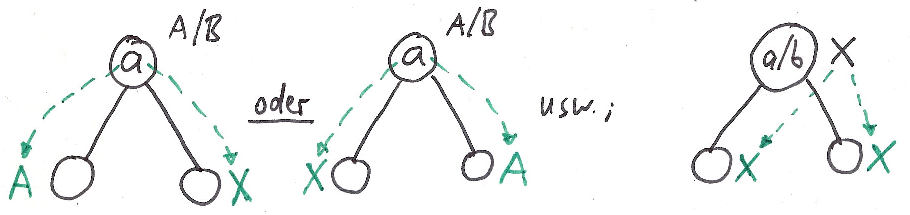
\includegraphics[scale=.5]{img/beispielautomaten_2.pdf}
        \end{center}
      \end{small}

      \par\smallskip
      $L_\omega(\Aut{A})$ $=$
      \only<.|handout:0>{?}%
      \uncover<+->{$\{t \mid \text{$t$ hat mind.\ einen Pfad mit $\infty$ vielen $a$'s}\}$}
      \par\bigskip
    \item<+->
      derselbe NBBA, aber mit $F=\{B,X\}$
      \par\smallskip
      $L_\omega(\Aut{A})$ $=$
      \only<.|handout:0>{?}%
      \uncover<+->{$\{t \mid \text{$t$ hat mind.\ einen Pfad mit $\infty$ vielen $b$'s}\}$}
      \par\bigskip
    \item<+->
      derselbe NBBA, aber mit $F=\{X\}$%
      \uncover<7->{:\qquad $L_\omega(\Aut{A}) = \emptyset$}
      \par\smallskip
      \only<5-6|handout:0>{$L_\omega(\Aut{A})$ $=$ }%
      \only<5|handout:0>{?}%
      \only<6|handout:0>{$\emptyset$}%
%           \par\medskip
    \item<7->
      derselbe NBBA, aber mit $F=\{A,B\}$%
%           \uncover<0|handout:1>{:\hfill $L_\omega(\Aut{A}) = \emptyset$}
%           \par\smallskip
      \only<7-8|handout:0>{:\quad $L_\omega(\Aut{A})$ $=$ }%
      \only<7|handout:0>{?}%
      \only<8|handout:0>{$\emptyset$}%
      \uncover<0|handout:1>{\phantom{$()$}}%
  \end{Itemize}%
  \alt<1-4,7-8|handout:1>{\vspace*{-3.2pt}}{\vspace*{-16.8pt}}%

  \note{%
    \textbf{16:24}
    
    \parII
    1.\ Bsp.:~ lies \textbf{spaltenweise!}
    
    \par
  }
\end{frame}

% ------------------------------------------------------------------------------------------
\begin{frame}
  \frametitle{Beispiele (Muller)}
  \label{fra:beispiele_muller}

  \begin{Itemize}
    \item<+->
      NMBA $\Aut{A}=(\{A,B\},~\{a,b\},~\Delta,~\{A\},~\{\{A\}\})$ mit %\Tafel
      \[
        \Delta = \{~(A,a,A,A),~(B,a,A,A),~(A,b,B,B),~(B,b,B,B)~\}
      \]
      Skizze:
      \par\vspace*{-1.4\baselineskip}
      \begin{center}
        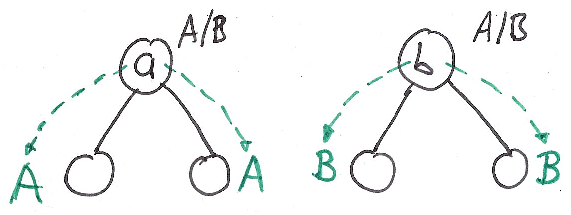
\includegraphics[scale=.45]{img/beispielautomaten_1.pdf}
      \end{center}

      \par\vspace*{-.4\baselineskip}
      $L_\omega(\Aut{A})$ $=$
      \only<.|handout:0>{?}%
      \uncover<+->{$\{t \mid \text{jeder Pfad hat endlich viele $b$'s}\}$ (!)}
      \par\medskip
    \item<+->
      derselbe NMBA, aber mit $F=\{\{B\}\}$
      \par\smallskip
      $L_\omega(\Aut{A})$ $=$
      \only<.|handout:0>{?}%
      \uncover<+->{$\{t \mid \text{jeder Pfad hat endlich viele $a$'s}\}$}
      \par\medskip
    \item<+->
      derselbe NMBA, aber mit $F=\{\{A,B\}\}$
      \par\smallskip
      $L_\omega(\Aut{A})$ $=$
      \only<.|handout:0>{?}%
      \uncover<+->{$\{t \mid \text{jeder Pfad hat $\infty$ viele $a$'s und $\infty$ viele $b$'s}\}$}
      \par\medskip
    \item<+->
      derselbe NMBA, aber mit $F=\{\{A\},\{B\}\}$
      \par\smallskip
      $L_\omega(\Aut{A})$ $=$
      \mbox{%
        \only<.|handout:0>{?}%
        \uncover<+->{$\{t \mid \text{jeder Pfad hat endl.\ viele $b$'s \emph{oder} endl.\ viele $a$'s}\}$}%
        \hspace*{-5mm}%
      }
  \end{Itemize}

  \note{%
    \textbf{16:28}
    
    \par
  }
\end{frame}
  
% ------------------------------------------------------------------------------------------
\begin{frame}
  \frametitle{Beispiel (Parität)}

    \Bmph{Zur Erinnerung:}
    \par\smallskip
    \begin{block}{}
      Run $r$ ist erfolgreich, wenn für alle Pfade $\pi \subseteq T$ gilt:
      \[
        \min\{c(q) \mid q \in \Inf(r,\pi)\} \text{~ist gerade}
      \]      
    \end{block}

    \par\bigskip
    \uncover<2->{%
      NPBA $\Aut{A}=(\{A,B\},~\{a,b\},~\Delta,~\{A\},~c)$ mit %\Tafel
      %
      \begin{align*}
        \Delta & = \{~(A,a,A,A),~(B,a,A,A),~(A,b,B,B),~(B,b,B,B)~\} \\[4pt]
        c(A)   & = 1                                                \\
        c(B)   & = 2
      \end{align*}
      %
      \vspace*{-4.4\baselineskip}
      \begin{center}
        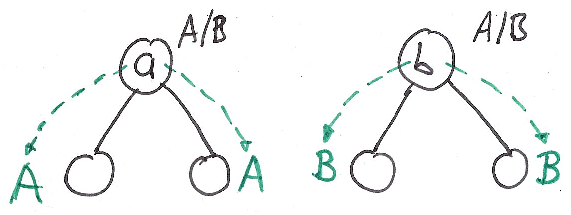
\includegraphics[scale=.45]{img/beispielautomaten_1.pdf}
      \end{center}
      %
      $L_\omega(\Aut{A})$ $=$
      \only<2|handout:0>{?}%
      \uncover<3>{$\{t \mid \text{jeder Pfad hat endlich viele $a$'s}\}$}
    }

  \note{%
    \textbf{16:32}
        
    \par
  }
\end{frame}

%% ------------------------------------------------------------------------------------------
%\begin{frame}
%  \frametitle{Büchi- versus Muller-Erkennbarkeit}
%  
%  \begin{Satz}
%    \begin{Enumerate}
%      \item
%        Jede Büchi-erkennbare Sprache ist Muller-erkennbar.
%      \item
%        \Emph{Nicht jede} Muller-erkennbare Sprache ist Büchi-erkennbar.
%    \end{Enumerate}
%    \label{thm:buchi_vs_muller}
%    \par\vspace*{-.4\baselineskip}
%  \end{Satz}
%
%  \par\medskip
%  \uncover<2->{%
%    \Bmph{Beweis.}
%    \begin{Enumerate}
%      \item
%        Wie im letzten Kapitel.
%      \item<3->
%        Idee:
%        \begin{Itemize}
%          \item
%            Betrachten $L = \{t \mid \text{jeder Pfad in $t$ hat endlich viele $a$'s}\}$;\\
%            nehmen an, $L$ werde von NBBA $\Aut{A}$ mittels Run $r$ erkannt
%          \item
%            Bestimme Baum $t \in L$ und Pfad, auf dem zwischen zwei Besuchen
%            \emph{desselben} akzeptierenden Zustandes ein $a$ auftritt
%          \item
%            "`Pumpe"' $t,r$ so auf, dass dieser Teilpfad sich $\infty$ oft wiederholt
%          \item[\dred{\lightning}]
%            Neuer Baum wird akzeptiert, aber neuer Pfad hat $\infty$ viele $a$'s
%        \end{Itemize}
%        \par\smallskip
%        Details: s.\ Tafel \Tafel~~~~
%    \end{Enumerate}
%  }
%  \uncover<3->{%
%    \par\vspace*{-1.3\baselineskip} \qed%
%  }
%
%  \note{%
%    \textbf{16:35 bis 16:55, 5\,min Pause}
%    
%    \parI
%    TODO:~ mehr vom Beweishergang auf Folie tun, weniger Tafelanschrieb!
%    
%    \par
%  }
%\end{frame}
%
% ------------------------------------------------------------------------------------------
\begin{frame}
  \frametitle{Büchi- versus Muller-Erkennbarkeit}
  
  \begin{Satz}
    \begin{Enumerate}
      \item
        Jede Büchi-erkennbare Sprache ist Muller-erkennbar.
      \item
        \Emph{Nicht jede} Muller-erkennbare Sprache ist Büchi-erkennbar.
    \end{Enumerate}
    \label{thm:buchi_vs_muller}
    \par\vspace*{-.4\baselineskip}
  \end{Satz}

  \par\medskip
  \uncover<2->{%
    \Bmph{Beweis.}
    \begin{Enumerate}
      \item
        Wie im letzten Kapitel.
        \par\medskip
      \item<3->
        Betrachten $L = \{t \mid \text{jeder Pfad in $t$ hat endlich viele $a$'s}\}$
        \par\medskip
        $L$ ist Muller-erkennbar (siehe Bsp.\ auf Folie~\ref{fra:beispiele_muller})
        \par\medskip
        Müssen zeigen: $L$ nicht Büchi-erkennbar
    \end{Enumerate}
  }

  \note{%
    \textbf{16:35}
    
    \par
  }
\end{frame}

% ------------------------------------------------------------------------------------------
\begin{frame}
  \frametitle{Büchi- versus Muller-Erkennbarkeit}
  
  \Bmph{Zu zeigen:}~~
  $L = \{t \mid \text{jeder Pfad in $t$ hat endlich viele $a$'s}\}$ \\
  nicht Büchi-erkennbar.
  
  \par\bigskip
  \uncover<2->{%
    Nehmen an, es gebe NBBA $\Aut{A} = (Q,\Sigma,\Delta,I,F)$ mit $L_\omega(\Amc) = L$.
  }
  
  \par\medskip
  \uncover<3->{%
    O.\,B.\,d.\,A.\ sei $I = \{q_0\}$.\qquad Sei $n := |F|$.
  }
  
  \par\bigskip
  \uncover<4->{%
    \Bmph{Idee:}~
    %
    \begin{Itemize}
      \item
        Bestimme Baum $t \in L$ mit Run $r$ und Pfad, auf dem zwischen 2~Besuchen
        \emph{desselben} akzeptierenden Zustandes ein $a$ auftritt
      \item
        "`Pumpe"' $t,r$ so auf, dass dieser Teilpfad sich $\infty$ oft wiederholt
      \item[\dred{\lightning}]
        Neuer Baum wird akzeptiert, aber neuer Pfad hat $\infty$ viele $a$'s
    \end{Itemize}
  }

  \note{%
    \textbf{16:36}
    
    \par
  }
\end{frame}

% ------------------------------------------------------------------------------------------
\begin{frame}
  \frametitle{Büchi- versus Muller-Erkennbarkeit}

  Betrachte Baum $t \in L$ mit
  \hfill
  $
    t(p) = a \quad\text{gdw.}\quad p \in \displaystyle\bigcup_{i=1,\dots,n} (1^+0)^i,
  $
  
  \par\medskip
  \uncover<2->{%
    d.\,h.\ $t$ enthält ein $a$ an allen Positionen, die man erreicht, \\
    wenn man bei der Wurzel startet und bis zu $n$-mal wie folgt läuft:
    %
    \begin{itemize}
      \item
        einmal oder mehrmals zum rechten Kind (beliebig oft)
      \item
        einmal zum linken Kind\quad ("`Linksschritt"')
    \end{itemize}
  }
  %
  \uncover<3->{%
    An den übrigen Positionen enthält $t$ ein $b$.
  }
  
  \par\medskip
  \uncover<4->{%
    \Bmph{Skizze:}
    \qquad
    \begin{tikzpicture}[%
      node distance=12mm,>=Latex,baseline=-4pt,
      every node/.style={circle,draw=none,fill=none,inner sep=.4mm,minimum size=4mm},
      every edge/.style={draw=black,thick}
    ]
      \node (00)                                {\footnotesize $b$};
      \node[below right=0mm and 3mm of 00] (01) {\footnotesize $b$};
      \node[below right=0mm and 3mm of 01] (02) {\footnotesize $b$};
      \node[below left =0mm and 3mm of 02] (10) {\small \Emph{$a$}};
      \node[below right=0mm and 3mm of 10] (11) {\footnotesize $b$};
      \node[below right=0mm and 3mm of 11] (12) {\footnotesize $b$};
      \node[below left =0mm and 3mm of 12] (20) {\small \Emph{$a$}};
      \node[below right=0mm and 3mm of 20] (21) {};
      
      \path[-]
        (00) edge (01)
        (01) edge[draw=none] node [sloped,pos=.6] {\scalebox{.8}[1]{{\footnotesize $\cdots$}}} (02)
        (02) edge (10)
        (10) edge (11)
        (11) edge[draw=none] node [sloped,pos=.6] {\scalebox{.8}[1]{{\footnotesize $\cdots$}}} (12)
        (12) edge (20)
        (20) edge[draw=none] node [sloped,pos=.6] {\scalebox{.8}[1]{{\footnotesize $\cdots$}}} (21)
        ;
    \end{tikzpicture}
    %
%    \raisebox{-2.5\baselineskip}{%
    \raisebox{-.7\baselineskip}{%
      $\left.\rule{0pt}{1.4\baselineskip}\right\}$
      \begin{tabular}{@{}l@{}}
        bis zu \\
        $n$-mal
      \end{tabular}
    }%
  }
  
  \par\medskip
  \uncover<5->{%
    Klar:~ $t \in L$.\qquad Sei $r$ ein erfolgreicher Run.
  }

  \par\medskip
  \uncover<6->{%
    Details des Pumpens: s.\ Tafel \Tafel~~~~
    \par\vspace*{-\baselineskip} \qed%
  }

  \note{%
    \textbf{16:38 bis 16:50, 5\,min Pause}
    
    \parI
    Man beachte:~ $a$'s tauchen in \emph{beliebiger Tiefe} auf, \\
    aber auf jedem Pfad nur auf den ersten $n$ Linksschritten.
    
    \parI
    Dadurch hat jeder Pfad nur max.\ $n$ $a$'s, also endlich viele.
    
    \par
  }
\end{frame}

% ------------------------------------------------------------------------------------------
\begin{frame}
  \frametitle{Folgerung aus dem Beweis von Satz \ref{thm:buchi_vs_muller}}

  \begin{Folgerung}
    Die Klasse der Büchi-erkennbaren Baumsprachen ist\\
    \Emph{nicht} abgeschlossen unter
    \only<1|handout:0>{?}%
    \uncover<2->{Komplement.}
    \label{cor:Buchi_erkennbar_nicht_unter_Komplement_abgeschlossen}
  \end{Folgerung}

  \par\bigskip
  \uncover<3->{%
    Man kann Satz \ref{thm:buchi_vs_muller} stärker formulieren (ohne Beweis):

    \par\medskip
    \begin{Satz}
      Die Menge der Baumsprachen, die Muller-, aber nicht Büchi-erkennbar sind, ist
      \[
        \{L_\triangle \mid L \text{ ist NBA-erkennbar, aber nicht DBA-erkennbar}\}.
      \]
    \end{Satz}
  }

  \par\medskip
  \uncover<3->{%

    \begin{small}
      ($L \subseteq \Sigma^\omega$ ist eine $\omega$-Sprache;
      \par\smallskip
      $L_\triangle$ $=$ Menge aller $\Sigma$-Bäume,
      deren Beschriftung entlang \emph{jedes} Pfades in $L$ \\
      \hspace*{\fill} liegt)
      \par
    \end{small}
  }

  \note{%
    \textbf{16:55}
    
    \parI
    \textbf{Vor Satz 4.14 sagen:}~ Anfang des letzten Beweises erinnert nicht ohne Grund
    an Beweis der Ungleichmächtigkeit von DBAs und NBAs
    
    \par
  }
\end{frame}

% ------------------------------------------------------------------------------------------
\begin{frame}
  \frametitle{Paritäts- versus Muller-Erkennbarkeit}

  \begin{Satz}
    \begin{Enumerate}
      \item
        Jede paritäts-erkennbare Sprache ist Muller-erkennbar.
      \item
        Jede Muller-erkennbare Sprache ist paritäts-erkennbar.
    \end{Enumerate}
    \label{thm:muller_vs_paritaet}
    \par\vspace*{-.2\baselineskip}
  \end{Satz}

  \par\medskip
  \uncover<2->{%
    \Bmph{Beweis.}
    \begin{Enumerate}
      \item
        Wie im letzten Kapitel.
      \item<3->
        Sei $\Amc = (Q,\Sigma,\Delta,I,\Fmc)$ NMBA, mit \\
        $I = \{q_0\}$ und $\Fmc=\{F\}$ (o.\,B.\,d.\,A.)\quad sowie $n := |Q|$.
        \par\medskip
        \uncover<4->{%
          \Bmph{Gesucht:}~ äquivalenter NPBA $\Amc'$
        }
        \par\smallskip
        \uncover<5->{%
          \Bmph{Idee:}~ $\Aut{A}'$ soll \dots
          \begin{Itemize}
            \item
              "`sich merken"', in welcher Reihenfolge die $n$ Zustände zuletzt gesehen wurden (Permutation $q_1\cdots q_n$ von $Q$)
            \item<6->
              sicherstellen, dass ab einem gewissen Zeitpunkt 
              genau die Zustände aus $F$ dauerhaft am Ende der Permutation stehen
          \end{Itemize}
        }
    \end{Enumerate}
  }

  \note{%
    \textbf{16:57}
    
    \par
  }
\end{frame}

% ------------------------------------------------------------------------------------------
\begin{frame}
  \frametitle{Details der Konstruktion (1)}

  Sei $\Aut{A} = (Q,\Sigma,\Delta,\{q_0\},F)$ NMBA mit $|Q|=n$.
  \par\smallskip
  Konstruieren NPBA $\Aut{A}' = (Q',\Sigma,\Delta',I',c)$ mit Zuständen
  \[
    \begin{array}{@{}l@{~}l@{~}l}
      Q' = \{\auf q_1\cdots q_n,\,\ell\zu \mid & q_1\cdots q_n \text{ ist Permutation von $Q$}, &    \\
                                               & \ell \in \{1,\dots,n\}                         & \}
    \end{array}
  \]

  \Bmph{Idee:}
  \begin{Itemize}
    \item
      $q_n$ ist der zuletzt besuchte Zustand auf dem aktuellen Pfad,\\
      $q_{n-1}$ der zuletzt besuchte Zustand $\neq q_n$ usw.
    \item
      $\ell$ ist Position von $q_n$ in der vorangehenden Permutation
  \end{Itemize}

  \par\smallskip
  Skizze: siehe Tafel \Tafel

  \note{%
    \textbf{16:59}
    
    \par
  }
\end{frame}

% ------------------------------------------------------------------------------------------
\begin{frame}
  \frametitle{Details der Konstruktion (2)}

  Zeigen zunächst folgende \Bmph{Hilfsaussage (HA)} über Zustände von $\Aut{A}'$

  \par\bigskip
  \begin{block}{}
    Sei $q_1q_2q_3\dots$ eine Folge von Zuständen aus $Q$; \\
    sei $s_1s_2s_3\dots$ die zugehörige Folge von Zuständen aus $Q'$\\
    \quad~~ mit $s_1 = \auf t_1\cdots t_{n-1}q_1,\,1\zu$ und $s_i = \auf \text{perm}_i,\ell_i\zu$ für alle $i \geqslant 0$.

    \par\bigskip
    Dann gilt $\text{Inf}(q_1q_2q_3\dots) = S$ mit $|S|=k$ gdw.\
    \begin{Enumerate}
      \item
        Für endlich viele $i$ ist $\ell_i \leqslant n-k$\quad und
      \item
        Für unendlich viele $i$ gilt:
        \begin{Itemize}
          \item[(a)]
            $\ell_i = n-k+1$\quad und
          \item[(b)]
            Die Menge der Zustände in den Positionen $\underbrace{n-k+1,\dots,n}_{\text{letzte $k$ Positionen}}$\\[-12pt]
            in $\text{perm}_i$ ist $S$
        \end{Itemize}
    \end{Enumerate}
  \end{block}

  \par\bigskip
  \Bmph{Beweis der Hilfsaussage:}
  siehe Tafel \Tafel

  \note{%
    \textbf{17:06 bis 17:11\quad Tafelanschrieb nur, wenn viel mehr Zeit!}
    
    \par
  }
\end{frame}

% ------------------------------------------------------------------------------------------
\begin{frame}
  \frametitle{Details der Konstruktion (3)}

  Können nun Konstruktion fortsetzen:
  \begin{small}
    \[
      \begin{array}{@{}r@{~}c@{~}l@{}}
        I'        & = & \Big\{\auf t_1\cdots t_{n-1}q_0,\,1\zu \mid t_1\cdots t_{n-1} \text{ ist Perm.\ von } Q\setminus\{q_0\}\Big\} \\[10pt]
        \uncover<2->{%
          \Delta' & = & \Big\{\Big(\auf i_1\cdots i_{n-1}i,\,\ell\zu,~ a,~ \auf i'_1\cdots i'_{n-1}i',\,\ell'\zu,~ \auf i''_1\cdots i''_{n-1}i'',\,\ell''\zu\Big) \mid \\
                  &   & \text{%
                          \parbox{.87\textwidth}{%
                            \begin{Itemize}
                              \item
                                $(i,a,i',i'') \in \Delta$
                              \item
                                $i_1'\cdots i_{n-1}'$ entsteht aus $i_1\cdots i_{n-1}i$ durch Löschen von $i'$
                              \item
                                $i_1''\cdots i_{n-1}''$ entsteht aus $i_1\cdots i_{n-1}i$ durch Löschen von $i''$
                              \item
                                $\ell'$ $=$ Position von $i'$ in $i_1\cdots i_{n-1}i$
                                \vspace*{-4pt}
                              \item
                                $\ell''$ $=$ Position von $i''$ in $i_1\cdots i_{n-1}i$ \hspace*{\fill} $\Big\}$
                            \end{Itemize}
                          }
                        } \\[10pt]
        }
        \uncover<3->{%
          c(s)    & = & \begin{cases}
                          2\ell   & \text{falls } s=\auf q_1\cdots q_n,\,\ell\zu \text{ und } \{q_\ell,\dots,q_n\} = F \\
                          2\ell+1 & \text{falls } s=\auf q_1\cdots q_n,\,\ell\zu \text{ und } \{q_\ell,\dots,q_n\} \neq F
                        \end{cases}
        }
      \end{array}
    \]
  \end{small}

  \par\smallskip
  \uncover<4->{%
    Beweis der Korrektheit: siehe Tafel \Tafel~~~~
    \par\smallskip
    \vspace*{-1.15\baselineskip}\qed
  }

  \note{%
    \textbf{17:11 bis 17:29;\quad (wenn Zeit knapp, dann ohne Tafelanschrieb)}
    
    \parI
    (!) Wahl der Akzeptanzbedingung wird nur durch Beweis so richtig klar \dots

    \par
  }
\end{frame}

% ------------------------------------------------------------------------------------------
\begin{frame}
  \frametitle{Abschlusseigenschaften}
  
  \begin{Satz}
    Die Klasse der \dots
    \begin{Enumerate}
      \item
        Büchi-erkennbaren Sprachen ist abgeschlossen unter $\cup$ und $\cap$,\\
        aber nicht unter $\overline{\phantom{o}}$.
      \item
        Muller-erkennbaren Sprachen ist abgeschlossen unter $\cup,\cap,\overline{\phantom{o}}$.
    \end{Enumerate}          
  \end{Satz}

  \par\bigskip
  \uncover<2->{%
%         \Bmph{Beweisidee:}
    \Bmph{Beweis:}
    \begin{Enumerate}
      \item
        $\cup\,\cap$ wie gehabt;\qquad $\overline{\phantom{o}}$ siehe Folgerung \ref{cor:Buchi_erkennbar_nicht_unter_Komplement_abgeschlossen}.
      \item
        $\cup\,\cap$ wie gehabt;
        \par\smallskip
        $\overline{\phantom{o}}$ 
%             anspruchsvoller Beweis, Resultat aus der Spieltheorie \Tafelvielleicht
        siehe nächsten Abschnitt % \Tafel~~~~
    \end{Enumerate}
    \par\vspace*{-1.4\baselineskip} \qed%
  }

  \note{%
    \textbf{17:29 bis 17:30 $\leadsto$ Ende Gelände}
    
    \par
  }
\end{frame}


  % ==============================================================================================
  % ==============================================================================================
  \section[Komplementierung]{Komplementierung} % von Automaten auf unendlichen Bäumen}
  % ------------------------------------------------------------------------------------------
\begin{frame}
  \frametitle{Überblick}

  \Bmph{Ziel dieses Abschnitts:}
  \par\smallskip
  Lösen Komplementierung mit Hilfe eines bekannten Resultates
  über Gewinnstrategien in einer bestimmten Art (abstrakter) Spiele

  \par\medskip
  \Bmph{Vorgehen:}
  \begin{Itemize}
    \item
      \mbox{\scalebox{.98}[1]{Ordnen jedem N\Emph{P}BA \Aut{A} und Baum $t$
      ein 2-Personen-Spiel \Game{A}{t} zu}\hspace*{-10mm}} \\
%      \par\smallskip
      {\small (Beschränkung auf N\Emph{P}BAs ist unerheblich, siehe Satz~\ref{thm:muller_vs_paritaet})}
%           \par\smallskip
    \item
      Dann wird leicht zu sehen sein:
      \par\smallskip
      $\Aut{A}$ akzeptiert $t$ ~$\Leftrightarrow$~ Spielerin 1 hat Gewinnstrategie in \Game{A}{t}
%           \par\smallskip
    \item
      Ein Resultat aus der Spieltheorie impliziert:
      \par\smallskip
      In \Game{A}{t} hat immer \Emph{genau eine Spielerin eine Gewinnstrategie,}\\
      \Emph{die nicht vom bisherigen Spielverlauf abhängt}
%           \par\smallskip
    \item
%           Konstruieren $\Aut{A}'$ anhand der Gewinnstrategie von Spielerin 2;\\
%           zeigen: $L_\omega(\Aut{A}') = \overline{L_\omega(\Aut{A})}$
      Konstruieren $\Aut{A}'$, so dass gilt:
      \par\smallskip
      $\Aut{A}'$ akzeptiert $t$ ~$\Leftrightarrow$~ \Emph{Spielerin 2 hat Gewinnstrategie in \Game{A}{t}}
      \par\smallskip
      Dann folgt $L_\omega(\Aut{A}') = \overline{L_\omega(\Aut{A})}$
  \end{Itemize}
  

  \note{%
    \textbf{16:00}
    
    \par
  }
\end{frame}

% ------------------------------------------------------------------------------------------
\begin{frame}
  \frametitle{Intuitive Beschreibung des Spiels \Game{A}{t}}
  
  Zwei Spielerinnen \AUT (Automat), \PF (Pfadfinderin)
  \begin{Itemize}
    \item
      sind abwechselnd an der Reihe
    \item
      bewegen sich pro Runde 1 Schritt im Baum
      durch Markieren von Positionen mit Zuständen; zu Beginn: $(\varepsilon,q_I)$,~ $q_I \in I$
  \end{Itemize}

  \par\bigskip
  \uncover<2->{%
    In jeder Runde wählt
    \begin{Itemize}
      \item
        \mbox{\AUT eine Transition, die auf die markierte Position anwendbar ist\hspace*{-10mm}}
      \item
        \PF einen Kindknoten und verschiebt Markierung dorthin
    \end{Itemize}
  }

  \par\bigskip
  \uncover<3->{%
    Spiel läuft $\infty$ lange, erzeugt $\infty$ Folge $r=q_0q_1q_2$ von Zuständen\\
    (bestimmt durch die gewählten Transitionen)%
  }

  \par\bigskip
  \uncover<4->{%
    \AUT gewinnt, wenn $r$ der Akzeptanzbedingung von \Aut{A} entspricht;\\
    sonst gewinnt \PF

    \par%\smallskip
    \begin{footnotesize}
      \mbox{(d.\,h.\ \AUT versucht, \Aut{A} zum Akzeptieren zu bringen; \PF versucht das zu verhindern)\hspace*{-10mm}}
      \par
    \end{footnotesize}
  }

  \par\bigskip
  \uncover<5->{%
    Skizze: s.\ Tafel \Tafel
  }

  \note{%
    \textbf{16:03 bis 16:12}
    
    \parI
    $q_I$ bezeichne ab hier einen beliebigen Anfangszustand; \\
    brauchen "`$q_0$"' später noch anderweitig.
    
    \parII
    Es wird also ein Baumautomat mit \textbf{beliebiger Akzeptanzbedingung} (Büchi, Muller, whatever) zugrunde gelegt.
    
    \par
  }
\end{frame}

% ------------------------------------------------------------------------------------------
\begin{frame}
  \frametitle{Genaue Beschreibung des Spiels \Game{A}{t}}

  Spiel ist ein unendlicher Graph
  \begin{Itemize}
    \item<+->
      Knoten sind die \Bmph{Spielpositionen}:
      \begin{Itemize}
        \item
          für \AUT: $\{(p,q) \mid p \in \{0,1\}^*,~ q \in Q\}$~ (Positionen im Baum)
        \item
          für \PF: $\{(q,t(p),q_0,q_1) \in \Delta \mid p \in \{0,1\}^*\}$\quad (Transitionen)
      \end{Itemize}
      \par\smallskip
    \item<+->
      Kanten sind die möglichen \Bmph{Spielzüge}:
      \begin{Itemize}
%        \item
%%               für \AUT:
%          $(p,q) \to (q',t(p'),q_0,q_1)$, wenn $p=p'$ und $q=q'$
%        \item
%%               für \PF:
%          $(q,t(p),q_0,q_1) \to (p',q')$, wenn $q'=q_i$ und $p'=pi$ für ein $i$
        \item
          $(p,q) \to (q,t(p),q_0,q_1)$
        \item
          \begin{tabular}[t]{@{}l@{~}c@{~}l@{}}
            $(q,t(p),q_0,q_1)$ & $\to$ & $(p0,q_0)$ \\
                               & \hspace*{-12pt}\raisebox{4pt}{\turnbox{-25}{$\to$}} & $(p1,q_1)$
          \end{tabular}
      \end{Itemize}
      \par\smallskip
    \item<+->
      Startknoten: $(\varepsilon,q_I)$ für $q_I \in I$\quad (o.\,B.\,d.\,A.\ $I=\{q_I\}$)
  \end{Itemize}

  \par\bigskip
  \uncover<+->{%
    Jede mögliche $\infty$ Folge von Spielzügen entspricht\\
    einem $\infty$ Pfad im Spielbaum \Game{A}{t}
  }

  \par\bigskip
  \uncover<+->{%
    Knoten $v'$ \Bmph{erreichbar} von Knoten $v$:\\
    es gibt endliche Folge von Spielzügen von $v$ nach $v'$
  }

  \note{
    \textbf{16:12}
    
    \parII
    \textbf{Achtung:}~ Ab jetzt bezeichnet $p$ Positionen im Baum, nicht mehr Zustände!
    
    \par
  }
\end{frame}

% ------------------------------------------------------------------------------------------
\begin{frame}
  \frametitle{Spielstrategien}

  \Bmph{Strategie ab Spielposition $v$} für Spielerin $X \in \{\AUT,\PF\}$:
  \par\smallskip
  Funktion, die jeder Zugfolge $v\dots v'$ mit $v'$ Spielposition für $X$ \\
  einen in $v'$ möglichen Zug zuweist
  \par%\smallskip
  \begin{footnotesize}
    (legt fest, welchen Zug $X$ in jeder von $v$ aus erreichbaren Spielposition macht)
    \par
  \end{footnotesize}

  \par\bigskip
  \uncover<2->{%
    \Bmph{Gewinnstrategie} für Spielerin $X \in \{\AUT,\PF\}$:
    \par\smallskip
    Strategie, die sicherstellt, dass $X$ gewinnt,\\
    \emph{unabhängig} von den Zügen der Gegenspielerin \Tafel
  }

  \par\bigskip
  \uncover<3->{%
    \Bmph{gedächtnislose Strategie:}
    \par\smallskip
    Strategie, die nur von $v'$ abhängt, nicht von den vorigen Positionen
  }

  \note{
    \textbf{16:17 bis 16:26}
    
    \par
  }
\end{frame}

% ------------------------------------------------------------------------------------------
\begin{frame}
  \frametitle{Akzeptanz mittels Gewinnstrategien}

  \begin{Lemma}
    Seien $\Aut{A} = (Q,\Sigma,\Delta,\{q_I\},c)$ ein NPBA und $t$ ein $\Sigma$-Baum.\\ Dann gilt:
    \par\smallskip
    $t \in L_\omega(\Aut{A})$ ~$\Leftrightarrow$~ \AUT hat Gewinnstrategie in $\Game{A}{t}$ ab Position $(\varepsilon,q_I)$%
    \label{lem:akzeptanz_vs_gewinnstrategien}%
%         \par\vspace*{-.4\baselineskip}
  \end{Lemma}

  \par\bigskip
  \uncover<2->{%
    \Bmph{Beweis:} 

    \par\smallskip
    Konstruiere Gewinnstrategie direkt aus einem erfolgreichen Run\\
    und umgekehrt

%    \par\medskip
%    Details: s.\ Tafel \Tafel~~~~
%    \par\vspace*{-.95\baselineskip}\qed
  }

  \note{
    \textbf{16:26}
    
%    \parII
%    Nach wie vor beliebige Akzeptanzbedingung (deshalb N\textbf{x}BA)
    
    \par
  }
\end{frame}

% ------------------------------------------------------------------------------------------
\begin{frame}
  \frametitle{Akzeptanz mittels Gewinnstrategien}
  
  \begin{block}{}
    \Bmph{"`$t \in L_\omega(\Aut{A})$ ~$\Rightarrow$~ \AUT hat Gewinnstrategie in $\Game{A}{t}$ ab Position $(\varepsilon,q_I)$"'}
  \end{block}
  
  \parII
  Gelte $t \in L_\omega(\Aut{A})$ und sei $r$ erfolgreicher Run von $\Aut{A}$ auf $t$.
  
  \par
  Konstruiere Gewinnstrategie für \AUT wie folgt aus $r$.
  %
  \begin{Itemize}
    \item<2->
      in Startposition $(\varepsilon,q_I)$ wähle
      $(r(\varepsilon),t(\varepsilon),r(0),r(1))$
    \item<3->
      in allen anderen Spielpos.\ $(p,q)$ wähle
      $(q,t(p),r(p0),r(p1))$
  \end{Itemize}
  
  \parI
  \uncover<4->{%
    Wenn \AUT diese Strategie befolgt,
    dann entspricht die im Spiel erzeugte Zustandsmenge
    einem Pfad in $r$.
  }

  \parII
  \uncover<5->{%
    Da $r$ erfolgreich, gewinnt \AUT nach Definition von $G_{\Aut{A},t}$\,.
  }

  \parII
  \uncover<6->{%
    \begin{block}{}
      \Bmph{"`\AUT hat Gewinnstrategie in $\Game{A}{t}$ ab Position $(\varepsilon,q_I)$ ~$\Rightarrow$~ $t \in L_\omega(\Aut{A})$"'}
    \end{block}
    \Tafel~~~~
    \par\vspace*{-.95\baselineskip}\qed
  }
  
  \note{
    \textbf{16:28 bis 16:38}
    
    \par
  }
\end{frame}

% ------------------------------------------------------------------------------------------
\begin{frame}
  \frametitle{Determiniertheit von Paritätsspielen}

  Klassisches Resultat aus der Spieltheorie, hier nicht bewiesen:

  \begin{Satz}[Emerson \& Jutla 1991, Mostowski 1991]
    Alle Paritätsspiele sind \Bmph{gedächtnislos determiniert}:\\
    genau eine der Spielerinnen hat eine \textup{gedächtnislose} Gewinnstrategie.%
    \label{thm:gedaechtnislos_determiniert}
  \end{Satz}

%       \begin{footnotesize}
%         E.\ A.\ Emerson und C.\ S.\ Jutla 1991,\quad A.\ Mostowski 1991 %\\
%         (ohne "`gedächtnislos"': D.\ A.\ Martin 1975)
%         \par
%       \end{footnotesize}

  \par\bigskip
  "`Paritätsspiel"' bezeichnet dabei 2-Personen-Spiele, die
  %
  \begin{Itemize}
    \item
      auf Graphen gespielt werden, \\
      deren Knoten mit natürlichen Zahlen markiert sind;
    \item
      als Gewinnbedingung für unendliche Spielverläufe \\
      die Paritätsbedingung verwenden.
  \end{Itemize}
  %
  \parI
  Für alle $\Aut{A}$ und $t$ ist $\Game{A}{t}$ ein Paritätsspiel.
  
  \note{
    \textbf{16:38}
    
    \par
  }
\end{frame}

% ------------------------------------------------------------------------------------------
\begin{frame}
  \frametitle{Determiniertheit von Paritätsspielen}

  Folgerung aus Satz~\ref{thm:gedaechtnislos_determiniert}:

  \begin{Folgerung}
    Seien $\Aut{A} = (Q,\Sigma,\Delta,\{q_I\},c)$ ein NPBA und $t$ ein $\Sigma$-Baum.
    \par\smallskip
%           Dann gibt es für jede Spielposition $v$ in \Game{A}{t}
%           eine gedächtnislose Gewinnstrategie für \AUT oder \PF.
%           \par\smallskip
%           Insbesondere gibt es ab $(\varepsilon,q_I)$
%           eine solche.
    Dann gibt es für jede Spielposition $v$ in \Game{A}{t}
    --- und insbesondere für $(\varepsilon,q_I)$ ---
    eine gedächtnislose Gewinnstrategie für \AUT oder \PF.%
    \label{cor:gedaechtnislose_determiniertheit}%
%           \par\vspace*{-.4\baselineskip}
  \end{Folgerung}

  \par\bigskip
  \uncover<2->{%
%         Das heißt (mit Lemma \ref{lem:akzeptanz_vs_gewinnstrategien}):
%         \par\smallskip
%         $t \in \overline{L_\omega(\Aut{A})}$ ~$\Leftrightarrow$~ \PF hat gedächtnislose GS ab $(\varepsilon,q_I)$ in $\Game{A}{t}$
% 
%         \par\bigskip
%         Benutzen diese nun, um einen NPBA für $\overline{L_\omega(\Aut{A})}$ zu konstruieren
    \begin{Folgerung}[aus Lemma \ref{lem:akzeptanz_vs_gewinnstrategien} und Folgerung \ref{cor:gedaechtnislose_determiniertheit}]
      $t \in \overline{L_\omega(\Aut{A})}$ ~$\Leftrightarrow$~ \PF hat gedächtnislose GS ab $(\varepsilon,q_I)$ in $\Game{A}{t}$
      \label{cor:gedaechtnislose_GS_fuer_PF}%
%           \par\vspace*{-.4\baselineskip}
    \end{Folgerung}

    \par%\bigskip
    \Emph{Ziel:} konstruieren NPBA, um deren Existenz zu testen
  }

  \note{
    \textbf{16:39 bis 16:41, 5min Pause}
    
    \par
  }
\end{frame}

% ------------------------------------------------------------------------------------------
\begin{frame}
  \frametitle{Gewinnbäume}

  Betrachten gedächtnislose Gewinnstrategien für \PF
  als Menge von Funktionen
  \[
    f_p : \Delta \to \{0,1\}\qquad \text{für jede Baumposition~} p \in \{0,1\}^*
  \]
  \Bmph{Idee:} $f_p$ weist jeder Transition, die \AUT in Baumposition $p$ wählt,
  einen Spielzug (Richtung 0/1) zu

  \par\bigskip
  \uncover<2->{%
    \begin{Itemize}
      \item
        Sei $F$ die Menge dieser Funktionen
      \item
        Ordnen die $f_p$ in einem \Bmph{$F$-Baum} $s$ an\quad (Strategiebaum)
    \end{Itemize}
  }

  \par\bigskip\vspace*{-.6pt}
  \uncover<3->{%
    \Bmph{PF-Gewinnbaum} für $t$:\\
    ein $F$-Baum, der eine Gewinnstrategie für \PF in \Game{A}{t} kodiert
  }

  \par\medskip
  \uncover<4->{%
    \begin{Folgerung}[aus Folgerung \ref{cor:gedaechtnislose_GS_fuer_PF}]
      $t \in \overline{L_\omega(\Aut{A})}$ ~$\Leftrightarrow$~ es gibt einen \PF-Gewinnbaum für $t$%
      \label{cor:Gewinnbaum_fuer_PF}%
%           \par\vspace*{-.4\baselineskip}
    \end{Folgerung}

    \par%\bigskip
    \mbox{\Emph{Neues Ziel:} bauen NPBA, um Existenz \PF-Gewinnbaum zu testen\hspace*{-10mm}}
  }

  \note{
    \textbf{16:46 bis 16:49}
    
    \par
  }
\end{frame}

% ------------------------------------------------------------------------------------------
\begin{frame}
  \frametitle{Existenz von PF-Gewinnbäumen (\PF-GB)}

  Sei $\Aut{A} = (Q,\Sigma,\Delta,\{q_I\},c)$ ein NPBA und $t$ ein $\Sigma$-Baum
  \par\smallskip
  \Emph{Zwischenziel:} Prüfen, ob gegebener $F$-Baum $s$ \Emph{kein} \PF-GB ist

  \par\medskip
  \uncover<2->{%
    \Bmph{Idee:}
    \begin{Itemize}
      \item
        Benutzen NPA $\Aut{A}'$\qquad \Emph{($\omega$-Wortautomat)}
      \item
        $\Aut{A}'$ prüft für jeden Pfad $\pi$ in t und jeden möglichen Spielzug von \AUT
        separat, ob Akzeptanzbedingung von \Aut{A} erfüllt ist
      \item[$\leadsto$]
        $\Aut{A}'$ akzeptiert $\geqslant 1$ Pfad ~$\Leftrightarrow$~ $s$ ist kein \PF-Gewinnbaum für $t$ 
    \end{Itemize}
  }

  \par\bigskip
  \uncover<3->{%
    Sei $\pi \in \{0,1\}^\omega$ ein Pfad mit $\pi=\pi_1\pi_2\pi_3\dots$
    
    \parI
    $\Aut{A}'$ arbeitet auf Wörtern der folgenden Form:
    \[
%           \Big(s(\varepsilon), t(\varepsilon), \pi[1]\Big),~
%           \Big(s(\pi[1]), t(\pi[1]), \pi[2]\Big),~
%           \dots
      \Big\auf s(\varepsilon), t(\varepsilon), \pi_1\Big\zu~~
      \Big\auf s(\pi_1), t(\pi_1), \pi_2\Big\zu~~
      \Big\auf s(\pi_1\pi_2), t(\pi_1\pi_2), \pi_3\Big\zu~~
      \dots
    \]
    Sei \Bmph{\Lst} die Sprache aller dieser Wörter
  }

  \par\medskip
  \uncover<4->{%
    Beispiel: s.\ Tafel \Tafel
  }

  \note{
    \textbf{16:49 bis 16:58}
    
    \par
  }
\end{frame}

% ------------------------------------------------------------------------------------------
\begin{frame}
  \frametitle{Konstruktion des Wortautomaten für Gewinnbäume}

  Sei $\Aut{A} = (Q,\Sigma,\Delta,\{q_I\},c)$ ein NPBA und $t$ ein $\Sigma$-Baum
  \par\smallskip
  Konstruieren NPA $\Aut{A}' = (Q,\Sigma',\Delta',\{q_I\},c)$ wie folgt:
  \begin{Itemize}
    \item<2->
      $\Sigma' = \Big\{\auf f,a,i\zu ~\Big|~ f \in F,~ a \in \Sigma,~ i \in \{0,1\}\Big\}$
      \par\smallskip
    \item<3->
      $Q,c$ wie in \Aut{A}\quad {\footnotesize (wollen Akzeptanz von \Aut{A} prüfen)}
      \par\smallskip
    \item<4->
      $\Delta' = \Big\{\Big(q,~\auf f,a,i\zu,~q_i'\Big) ~\Big|~ \auf f,a,i\zu \in \Sigma',~ i \in \{0,1\},~$\\
      \hspace*{\fill} es gibt $\delta = (q,a,q_0',q_1') \in \Delta$ mit $f(\delta)=i\Big\}$
  \end{Itemize}

  \par\medskip
  \uncover<5->{%
    $\Aut{A}'$ prüft für \emph{jeden möglichen} Zug von \AUT,
    ob \AUT gewinnen kann
  }

  \par\medskip
  \uncover<6->{%
    \begin{lemma}
      $s$ ist ein \PF-Gewinnbaum für $t$
      ~$\Leftrightarrow$~
      $\Lst \cap L_\omega(\Aut{A}') = \emptyset$
      \label{lem:Gewinnbaum_mittels_Wortautomat}%
    \end{lemma}
  }

  \par\smallskip
  \uncover<7->{%
    \Bmph{Beweis:} s.\ Tafel \Tafel~~~
    \par\vspace*{-.95\baselineskip}\qed
  }

  \note{
    \textbf{16:58 $\to$ mit Beweis bis 17:30}
        
    \parII
    \textbf{Achtung:} $f \in F$ bedeutet "`Funktion aus der Menge aller Funktionen (Gewinnstrategien)"',
    nicht "`akzeptierender Zustand"'!
    
    \par
  }
\end{frame}


{
%   \setbeamertemplate{background}{{\Huge\Rewind\Rewind}}%
\usebackgroundtemplate{{\Huge\Rewind\Rewind}}%
%   \def\insertframenumber{\@arabic\c@framenumber}%
\def\insertframenumber{\relax}%
%   \AtBeginFrame{\addtocounter{framenumber}{-1}}%
%   \usebackgroundtemplate{{\Huge\Rewind\Rewind}}%
% ------------------------------------------------------------------------------------------
  \begin{frame}<handout:0>
    \frametitle{Komplementierung:~ Was bisher geschah \hfill \Rewind\Rewind}
    \addtocounter{framenumber}{-1}%

    \begin{Itemize}
      \item
        Gegeben: \Bmph{NPBA $\Autb{A}$} $= (Q,\Sigma,\Delta,\{q_I\},c)$
      \item
        Ordnen \Aut{A} und jedem \Bmph{Eingabebaum $t$} ein 2-Pers.-Spiel \Bmph{\Gameb{A}{t}} zu
      \item
        Spielerin \AUT wählt Transition für aktuelle Position in $t$;\\
        \PF wählt Kindsposition\quad ($\leadsto$ gibt schrittweise Pfad vor)
      \item
        \AUT gewinnt, wenn gespielter Pfad $c$ entspricht
    \end{Itemize}

    \begin{block}{Lemma~\ref{lem:akzeptanz_vs_gewinnstrategien}}
      $t \in L_\omega(\Aut{A})$ ~$\Leftrightarrow$~ \AUT hat Gewinnstrategie in $\Game{A}{t}$ ab Position $(\varepsilon,q_I)$%
    \end{block}

    \par\bigskip
    Mittels Resultat aus der Spieltheorie folgt:

    \begin{block}{Folgerung~\ref{cor:gedaechtnislose_GS_fuer_PF}}
      $t \in \overline{L_\omega(\Aut{A})}$ ~$\Leftrightarrow$~ \PF hat \Emph{gedächtnislose} GS ab $(\varepsilon,q_I)$ in $\Game{A}{t}$
    \end{block}

    \note{%
      \textbf{8:30}
      
      \par
    }
  \end{frame}

% ------------------------------------------------------------------------------------------
  \begin{frame}<handout:0>
    \frametitle{Komplementierung:~ Was bisher geschah \hfill \Rewind\Rewind}
    \addtocounter{framenumber}{-1}%

    \begin{Itemize}
      \item
        Betrachten gedächtnislose Gewinnstrategie für \PF als Menge $F$ von Funktionen
        \[
          f_p : \Delta \to \{0,1\}\qquad \text{für jede Baumposition~} p \in \{0,1\}^*
        \]
      \item
        Ordnen die $f_p$ in \Bmph{$F$-Baum $s$} an %(Strategiebaum)
        
        
%        \hfill ($F$ $\hat=$ alle $f_p$)
      \item
        \Bmph{\PF-Gewinnbaum:} $F$-Baum für eine Gewinnstrategie von \PF
    \end{Itemize}

    \par\bigskip
    Dann folgt sofort:

    \begin{block}{Folgerung~\ref{cor:Gewinnbaum_fuer_PF}}
      $t \in \overline{L_\omega(\Aut{A})}$ ~$\Leftrightarrow$~ es gibt einen \PF-Gewinnbaum für $t$%
    \end{block}

    \note{%
      \textbf{8:32}
      
      \parII
      $F$-Baum auch "`Strategiebaum"'; \\
      $F$ $\hat=$ alle $f_p$

      \par
    }
  \end{frame}

% ------------------------------------------------------------------------------------------
  \begin{frame}<handout:0>
    \frametitle{Komplementierung:~ Was bisher geschah \hfill \Rewind\Rewind}
    \addtocounter{framenumber}{-1}%

    Konstruieren NPA $\Aut{A}'$ ($\omega$-Wortautomat!), um \PF-Gewinnbäume zu erkennen:
    \begin{Itemize}
      \item
        Eingabewörter haben die Form
        \[
          \Big\auf s(\varepsilon), t(\varepsilon), \pi_1\Big\zu~~
          \Big\auf s(\pi_1), t(\pi_1), \pi_2\Big\zu~~
          \Big\auf s(\pi_1\pi_2), t(\pi_1\pi_2), \pi_3\Big\zu~~
          \dots
        \]
      \item
        Sei \Bmph{\Lst} die Menge aller solcher Wörter
    \end{Itemize}

    \par\bigskip
    Konstruktion von $\Aut{A}'$ stellt sicher:
%    \begin{center}
%      $s$ ist ein Gewinnbaum für $t$
%      ~$\Leftrightarrow$~
%      $\Lst \cap L_\omega(\Aut{A}') = \emptyset$
%    \end{center}
    \begin{block}{Lemma~\ref{lem:Gewinnbaum_mittels_Wortautomat}}
      $s$ ist ein \PF-Gewinnbaum für $t$
      ~$\Leftrightarrow$~
      $\Lst \cap L_\omega(\Aut{A}') = \emptyset$
    \end{block}
    
    \note{%
      \textbf{8:34}
      
      \par
    }
  \end{frame}
}



% ------------------------------------------------------------------------------------------
\begin{frame}
  \frametitle{Konstruktion des Komplementautomaten für \Aut{A}}

%       \begin{alertblock}{Gesucht {\small (siehe Folgerung \ref{cor:Gewinnbaum_fuer_PF})}}
%         NPBA $\Aut{B}$, der $t$ akzeptiert gdw.\ es einen Gewinnbaum für $t$ gibt 
%       \end{alertblock}
  \begin{alertblock}{}
    \Emph{Gesucht:}~ {\small (siehe Folgerung \ref{cor:Gewinnbaum_fuer_PF})}
    \par\smallskip
    NPBA $\Aut{B}$, der $t$ akzeptiert gdw.\ es einen \PF-Gewinnbaum für $t$ gibt 
  \end{alertblock}

  \par\smallskip
  \uncover<2->{%
    Wegen Lemma~\ref{lem:Gewinnbaum_mittels_Wortautomat} muss \Aut{B} akzeptieren ~gdw.~
    $
      \Lst \subseteq \overline{L_\omega(\Aut{A}')}
    $
  }

  \par\bigskip\smallskip
  \uncover<3->{%
    Konstruktion von \Aut{B} in 2 Schritten:
    
    \par\smallskip
    \Bmph{Schritt 1}
    \begin{Itemize}
      \item
        \mbox{Sei $\Aut{A}'' = (Q'', \Sigma', \Delta'', q_I'', c'')$ der \Emph{D}PA mit $L_\omega(\Aut{A}'') = \overline{L_\omega(\Aut{A}')}$\hspace*{-10mm}}
      \item
        $\Aut{A}''$ ist \Emph{deterministisch:}~ Safra-Konstruktion\\
        ($+$ Umwandlung zwischen den Automatentypen)
    \end{Itemize}
  }

  \par\medskip
  \uncover<4->{%
    \Bmph{Schritt 2}
    \par\smallskip
    \Aut{B} soll auf jedem Pfad von $t$
    \begin{Itemize}
      \item
        $\Aut{A}''$ laufen lassen
      \item
        und "`parallel"' dazu eine Strategie für \PF raten
    \end{Itemize}
  }

  \note{%
    \textbf{8:36 bis 8:40}
      
    \parII
    "`$\Lst \subseteq \overline{L_\omega(\Aut{A}')}$"':~
    ist äquivalent zu "`$\Lst \cap L_\omega(\Aut{A}') = \emptyset"'$ aus L.~\ref{lem:Gewinnbaum_mittels_Wortautomat}
    
    \parIII
    \textbf{Zu Schritt 1:} \\
    NPA $\to$ NMA $\to^*$ NBA ---Safra$\to^*$ DRA $\to$ DMA $\to^*$ DPA \\
    ${}^*$Resultate aus Vorlesung, exp. Blowup \\
    Es gibt effizientere direkte Konstruktion NPA $\to$ DPA (sage am Ende was dazu).
    
    \parIII
    \textbf{Zu Schritt 2:} \\
    $\Aut{A}''$ braucht ja als Eingabe Tripel, 1.\ Komponente $s(\cdot)$ aus Strategie. \\
    Diese Info wird schrittweise geraten.
    
    \par
  }
\end{frame}

% ------------------------------------------------------------------------------------------
\begin{frame}
  \frametitle{Konstruktion des Komplementautomaten für \Aut{A}}
  
  \Bmph{Idee:}~
  NPBA $\Bmc$ soll $\Amc''$ auf \Emph{jedem} Pfad simulieren, indem $\Bmc$
  %
  \begin{itemize}
    \item
      $s$ rät\quad (also pro Position $p$ ein $f_p$)
    \item
      sich ansonsten wie $\Amc''$ verhält, \\
      (also pro Position die Folgezustände $q_0,q_1$ gemäß $\Delta''$ setzt)
  \end{itemize}
  %
  $\Amc''$ deterministisch $\Rightarrow$ Zustand pro Position $p$ eindeutig bestimmt
  
  \parIII
  \uncover<2->{%
    \Bmph{Konstruktion von $\Autb{B} = (Q'', \Sigma, \Delta^{\text{neu}}, q_I'', c'')$:}
    \begin{Itemize}
      \item
        $Q'',q_I'',c''$ werden von $\Aut{A}''$ übernommen
      \item
        $\Delta^{\text{neu}} = \Big\{ (q,a,q_0,q_1) ~\Big|~ \text{es gibt } f \in F \text{ mit }$\\
        \hspace*{\fill}$\Big(q, \auf f,a,i\zu, q_i\Big) \in \Delta'' \text{ für } i=0,1\Big\}$
    \end{Itemize}
  }

  \par\vspace*{-.2\baselineskip}
  \uncover<3->{%
%    \Bmph{Es bleibt zu zeigen:}

%    \par\smallskip
    \begin{lemma}
      $t \in L_\omega(\Aut{B})$ ~gdw.~ es gibt $F$-Baum $s$ mit $\Lst \subseteq L_\omega(\Amc'')$
%      $L_\omega(\Aut{B}) = \overline{L_\omega(\Aut{A})}$
      \label{lem:Korrektheit_Komplementautomat}%
    \end{lemma}
  }

%  \parI
  %\vspace*{-\baselineskip}
  \uncover<4->{%
    \Bmph{Beweis:}~ siehe Tafel \Tafel~~~~
    \par\vspace*{-.95\baselineskip}\qed
  }
  
  \note{%
    \textbf{8:40 $\to$ bis 9:10}
    
    \parI
    DPA $\Amc''$ "`bezeugt"', dass $s$ \emph{kein} \PF-Gewinnbaum für $t$ ist
    
    \parII
    "`$\Aut{A}''$ deterministisch \dots"':~
    obwohl $\infty$ viele Pfade durch $p$ gehen!

    \parIII
    \uncover<2->{%
      $f \in F$:~
      Für \emph{jede mögliche} Funktion $f : \Delta \to \{0,1\}$~ ("`\dots\ $s$ rät"'!) \\
      und zugehörigen Übergang in $\Delta''$, ein neuer Übergang%
    }
    
    \parIII
    \uncover<3->{%
      Lemma ankündigen mit: "`es bleibt zu zeigen \dots"'%
    }
    
    \par
  }
\end{frame}

% ------------------------------------------------------------------------------------------
\begin{frame}
%       \frametitle{\dots}
  \begin{center}
    \begin{Large}
      \Gmph{\dots\ Es darf aufgeatmet werden \dots} \quad \dgre{\smiley}
    \end{Large}
  \end{center}
    
  \note{%
    \textbf{9:10}
    
    \parII
    Jetzt haben wir alles Technische geschafft und können das Hauptresultat sehr einfach beweisen.
    
    \parII
    Danach haben wir uns eine Pause verdient. :)
    
    \par
  }
\end{frame}

% ------------------------------------------------------------------------------------------
\begin{frame}
  \frametitle{Das Resultat}

  \begin{Satz}[Rabin 1969]
    Für jeden NPBA \Aut{A} gibt es einen NPBA \Aut{B}
    mit $L_\omega(\Aut{B}) = \overline{L_\omega(\Aut{A})}$.
  \end{Satz}

  \par\smallskip
  \uncover<2->{%
    \Bmph{Beweis:}
    \par\smallskip
    Für den bisher konstruierten NPBA \Aut{B} gilt:
%    Direkte Konsequenz aus Folg.~\ref{cor:Gewinnbaum_fuer_PF} und Lemmas~\ref{lem:Gewinnbaum_mittels_Wortautomat}, \ref{lem:Korrektheit_Komplementautomat} \qed
    \par\vspace*{-1.4\baselineskip}
    \begin{alignat*}{2}
      \Emph{$t \in L_\omega(\Autb{B})$} & ~~\text{gdw.}~~ \exists s \,.\, \Lst \subseteq L_\omega(\Amc'')           &\qquad  & \text{(Lemma~\ref{lem:Korrektheit_Komplementautomat})}\\
                                        & ~~\text{gdw.}~~ \exists s \,.\, \Lst \subseteq \overline{L_\omega(\Amc')} &        & \text{(Konstr.~$\Aut{A}''$)} \\
                                        & ~~\text{gdw.}~~ \exists s \,.\, \Lst \cap L_\omega(\Amc') = \emptyset     &        & \text{(Mengenlehre)} \\
                                        & ~~\text{gdw.}~~ \exists\, \text{\PF-Gewinnbaum $s$ für $t$}               &        & \text{(Lemma~\ref{lem:Gewinnbaum_mittels_Wortautomat})} \\
                                        & ~~\text{gdw.}~~ \Emph{$t \in \overline{L_\omega(\Autb{A})}$}              &        & \text{(Folg.~\ref{cor:Gewinnbaum_fuer_PF})}
    \end{alignat*}
    \qed
  }

  \note{%
    \textbf{9:10 bis 9:13}
    
    \parII
    Jetzt müssen wir nur noch alle Lemmas zusammentun und erhalten das Hauptresultat.
    
    \parII
    "`Konstr.~$\Aut{A}''$"':~ ist Komplementärautomat zu $\Aut{A}'$
    
    \parII
    \textbf{TODO:}~ Wenn Zeit ist, Beispiel für die Konstruktion vorführen \\
    (siehe Notizen in Sammlung nach T4.15, zweites$=$einfacheres Bsp.)
    
    \par
  }
\end{frame}

% ------------------------------------------------------------------------------------------
\begin{frame}
  \frametitle{Bemerkungen zur Komplexität der Konstruktion}

    Sei $n=|Q|$\quad (Anzahl der Zustände des NBPA \Aut{A}).
    
    \parI
    Dann hat der NPA $\Aut{A}'$ dieselben $n$ Zustände.
    
    \parI
    DPA $\Aut{A}''$ kann so konstruiert werden, dass $|Q''| \in O(2^{n \log n})$.
    
    \parI
    $\leadsto$ NBPA $\Aut{B}$ hat $O(2^{n \log n})$ Zustände.

  \note{%
    \textbf{9:13; auf Literatur verweisen, dann fertig? Oder noch Alternierung beginnen?}
    
    \parII
    Punkt 3 folgt \textbf{nicht} aus den Resultaten dieser Vorlesung.
    
    \parI
    Naives Vorgehen: \\
    NPA $\to$ NMA $\to^*$ NBA ---Safra$\to^*$ DRA $\to$ DMA $\to^*$ DPA \\
    ${}^*$Resultate aus Vorlesung, exp. Blowup \\
    Es gibt offenbar eine effizientere direkte Konstruktion NPA $\to$ DPA
    
    
    \par
  }
\end{frame}

%   % ------------------------------------------------------------------------------------------
%     \begin{frame}
%       \frametitle{\dots}
%       \dots
%       \note{~}
%     \end{frame}
% 


  \AtBeginSection{\relax}
%  % ==============================================================================================
%  % ==============================================================================================
%  \section*{Schlussbemerkungen}
%  % ------------------------------------------------------------------------------------------
\begin{frame}
  \frametitle{Abschließende Bemerkungen}

  \Bmph{Zusammenfassung}
  \begin{Itemize}
    \item
      NBBA sind schwächer als NMBA und NPBA
    \item
      Büchi-, Muller- und paritäts-erkennbare Sprachen sind
      abgeschlossen unter $\cup,\cap$ (leicht)
    \item
      Büchi-erkennbare Sprachen sind \emph{nicht}
      abgeschlossen unter $\overline{\phantom{\circ}}$
    \item
      Muller- und paritäts-erkennbare Sprachen \emph{sind}
      abgeschlossen unter $\overline{\phantom{\circ}}$ (anspruchsvoll, Spieltheorie)
    \item
      Komplementierung ist zentral im Beweis der Entscheidbarkeit
      der monadischen Logik zweiter Stufe\hfill {\footnotesize \Lit{(Kapitel 12 in LNCS 2500)}}
  \end{Itemize}
  \note{~}
\end{frame}

% ------------------------------------------------------------------------------------------
\begin{frame}
  \frametitle{Abschließende Bemerkungen}

  \Bmph{Ausblick}
  \begin{Itemize}
    \item
      Leerheitsproblem für NPBA ist entscheidbar;\\
      beste bekannte obere Schranke: $\text{UP} \cap \text{coUP}$ ($\subseteq \NP$)
      \par%\smallskip
      \hspace*{\fill}{\footnotesize \Lit{(Kapitel 8 in LNCS 2500)}}
    \item
      Verallgemeinerung des Nichtdeterminismus:\\
      alternierende Baumautomaten\hfill {\footnotesize \Lit{(Kapitel 9 in LNCS 2500)}}
  \end{Itemize}
  \note{~}
\end{frame}

% ------------------------------------------------------------------------------------------
\begin{frame}
  \frametitle{Das war \dots}
  \dots\ das Kapitel über Automaten auf unendlichen Bäumen.

  \par\bigskip
  \begin{center}
    \includegraphics[width=.8\textwidth]{img/pythagoras_tree_col_skewed.png}
%         *** REACTIVATE IMAGE ***
    \par
    \begin{footnotesize}
      Pythagoras-Baum. Quelle: Wikipedia, User Gjacquenot (Lizenz CC BY-SA 3.0)
      \par
    \end{footnotesize}
  \end{center}
  \note{~}
\end{frame}

% ------------------------------------------------------------------------------------------
\begin{frame}
  \frametitle{Was jetzt noch fehlt \dots}

  \begin{Itemize}
    \item
      kurze Nachbesprechung Vorlesungsevaluation
    \item
      Hinweise zu Fachgesprächen/mündl.\ Prüfung
  \end{Itemize}


  \par\bigskip
  \uncover<2->{%
    \begin{center}
      \begin{huge}
        \Emph{Vielen Dank für eure Teilnahme!}
        \par
      \end{huge}
    \end{center}
  }
  \note{~}
\end{frame}

%   % ------------------------------------------------------------------------------------------
%     \begin{frame}
%       \frametitle{\dots}
%       \dots
%       \note{~}
%     \end{frame}
%


%   % ------------------------------------------------------------------------------------------
%     \begin{frame}
%       \frametitle{\dots}
%       \dots
%       \note{~}
%     \end{frame}
% 
%   % ------------------------------------------------------------------------------------------
%     \begin{frame}
%       \frametitle{\dots}
%       \dots
%       \note{~}
%     \end{frame}
 


  % ==============================================================================================
  % ==============================================================================================
  \section*{}

  % ------------------------------------------------------------------------------------------
    \begin{frame}
      \frametitle{Literatur für diesen Teil (Basis, 1)}
      \begin{small}
        \begin{thebibliography}{99}
          \bibitem{Rog02}
            E.\ Grädel, W.\ Thomas, T.\ Wilke (Hrsg.).
            \newblock
            Automata, Logics, and Infinite Games.
            \newblock
            LNCS 2500, Springer, 2002, S. 43--60.
            \newblock
            Kapitel 6--9 über Paritätsspiele und Baumautomaten.\\
            \url{http://www.cs.tau.ac.il/~rabinoa/Lncs2500.zip}
            \newblock
            Auch erhältlich auf Anfrage in der BB Mathematik im MZH:\\
            \texttt{19h inf 001 k/100-2500}
          \bibitem{Bie09}
            Meghyn Bienvenu.
            \newblock
            Automata on Infinite Words and Trees.
            \newblock
            Vorlesungsskript, Uni Bremen, WS 2009/10.\\
            Kapitel 4.
            \newblock
            \url{http://www.informatik.uni-bremen.de/tdki/lehre/ws09/automata/automata-notes.pdf}
        \end{thebibliography}
        \par
      \end{small}
      \note{~}
    \end{frame}

  % ------------------------------------------------------------------------------------------
    \begin{frame}
      \frametitle{Literatur für diesen Teil (Basis, 2)}
      \begin{small}
        \begin{thebibliography}{99}
          \bibitem{BK08}
            Christel Baier, Joost-Pieter Katoen.
            \newblock
            Principles of Model Checking.
            \newblock
            MIT Press 2008.
            \newblock
            Abschnitt 6 "`Computation Tree Logic"'.
            \newblock
            SUB, Zentrale:
            \texttt{a inf 440 ver/782},~ \texttt{a inf 440 ver/782a}
          \bibitem{CGP99}
            Edmund M.\ Clarke, Orna Grumberg, Doron A.\ Peled.
            \newblock
            Model Checking.
            \newblock
            MIT Press 1999.
            \newblock
            Abschnitt 3 "`Temporal Logics"',\\
            Abschnitt 4 "`Model Checking"'.
%             Abschnitt 9.4 "`Translating LTL into Automata"'.
            \newblock
            SUB, Zentrale:
            \texttt{a\hfill inf\hfill 440\hfill ver/780(6)},\hfill\hfill  \texttt{a\hfill inf\hfill 440\hfill ver/780(6)a}
        \end{thebibliography}
        \par
      \end{small}
      \note{~}
    \end{frame}

  % ------------------------------------------------------------------------------------------
    \begin{frame}
      \frametitle{Literatur für diesen Teil (weiterführend)}
      \begin{small}
        \begin{thebibliography}{99}
          \bibitem{CD88}
            Edmund M.\ Clarke, I. A. Draghicescu
            \newblock
            Expressibility Results for Linear-Time and Branching-Time Logics
            \newblock
            REX Workshop 1988, S.\ 428--437.
            \newblock
            \url{https://doi.org/10.1007/BFb0013029}
        \end{thebibliography}
        \par
      \end{small}
      \note{~}
    \end{frame}


%   \AtBeginSection{\frame{\frametitle{Und nun \dots}\tableofcontents[currentsection]}}
  

%     % ------------------------------------------------------------------------------------------
%     \begin{frame}
%       \frametitle{Ausblick}
% 
%       \dots
%       
%       \par\bigskip
%       \uncover<2>{%
%         \begin{center}
%           \begin{Huge}
%             \dblu{\textbf{Thank you.}}
%           \end{Huge}
%         \end{center}
%       }
%     \end{frame}

%   % ==============================================================================================
%   % ==============================================================================================
%   \appendix
%   
%     % ------------------------------------------------------------------------------------------
%     \begin{frame}
%       \frametitle{\dots}
%       \dots
%     \end{frame}

\mode<presentation>{
  {   
    \setbeamercolor{background canvas}{bg=black}
    \begin{frame}<handout:0>[plain]{}
      \note{~}
    \end{frame}
  }
}

\end{document}
